% Options for packages loaded elsewhere
\PassOptionsToPackage{unicode}{hyperref}
\PassOptionsToPackage{hyphens}{url}
\PassOptionsToPackage{dvipsnames,svgnames,x11names}{xcolor}
%
\documentclass[
  10.5pt,
  letterpaper,
  DIV=11,
  numbers=noendperiod]{scrartcl}

\usepackage{amsmath,amssymb}
\usepackage{iftex}
\ifPDFTeX
  \usepackage[T1]{fontenc}
  \usepackage[utf8]{inputenc}
  \usepackage{textcomp} % provide euro and other symbols
\else % if luatex or xetex
  \usepackage{unicode-math}
  \defaultfontfeatures{Scale=MatchLowercase}
  \defaultfontfeatures[\rmfamily]{Ligatures=TeX,Scale=1}
\fi
\usepackage{lmodern}
\ifPDFTeX\else  
    % xetex/luatex font selection
\fi
% Use upquote if available, for straight quotes in verbatim environments
\IfFileExists{upquote.sty}{\usepackage{upquote}}{}
\IfFileExists{microtype.sty}{% use microtype if available
  \usepackage[]{microtype}
  \UseMicrotypeSet[protrusion]{basicmath} % disable protrusion for tt fonts
}{}
\makeatletter
\@ifundefined{KOMAClassName}{% if non-KOMA class
  \IfFileExists{parskip.sty}{%
    \usepackage{parskip}
  }{% else
    \setlength{\parindent}{0pt}
    \setlength{\parskip}{6pt plus 2pt minus 1pt}}
}{% if KOMA class
  \KOMAoptions{parskip=half}}
\makeatother
\usepackage{xcolor}
\usepackage[top=12mm, bottom=12mm, left=12mm, right=12mm]{geometry}
\setlength{\emergencystretch}{3em} % prevent overfull lines
\setcounter{secnumdepth}{-\maxdimen} % remove section numbering
% Make \paragraph and \subparagraph free-standing
\ifx\paragraph\undefined\else
  \let\oldparagraph\paragraph
  \renewcommand{\paragraph}[1]{\oldparagraph{#1}\mbox{}}
\fi
\ifx\subparagraph\undefined\else
  \let\oldsubparagraph\subparagraph
  \renewcommand{\subparagraph}[1]{\oldsubparagraph{#1}\mbox{}}
\fi


\providecommand{\tightlist}{%
  \setlength{\itemsep}{0pt}\setlength{\parskip}{0pt}}\usepackage{longtable,booktabs,array}
\usepackage{calc} % for calculating minipage widths
% Correct order of tables after \paragraph or \subparagraph
\usepackage{etoolbox}
\makeatletter
\patchcmd\longtable{\par}{\if@noskipsec\mbox{}\fi\par}{}{}
\makeatother
% Allow footnotes in longtable head/foot
\IfFileExists{footnotehyper.sty}{\usepackage{footnotehyper}}{\usepackage{footnote}}
\makesavenoteenv{longtable}
\usepackage{graphicx}
\makeatletter
\def\maxwidth{\ifdim\Gin@nat@width>\linewidth\linewidth\else\Gin@nat@width\fi}
\def\maxheight{\ifdim\Gin@nat@height>\textheight\textheight\else\Gin@nat@height\fi}
\makeatother
% Scale images if necessary, so that they will not overflow the page
% margins by default, and it is still possible to overwrite the defaults
% using explicit options in \includegraphics[width, height, ...]{}
\setkeys{Gin}{width=\maxwidth,height=\maxheight,keepaspectratio}
% Set default figure placement to htbp
\makeatletter
\def\fps@figure{htbp}
\makeatother

\usepackage{booktabs}
\usepackage{longtable}
\usepackage{array}
\usepackage{multirow}
\usepackage{wrapfig}
\usepackage{float}
\usepackage{colortbl}
\usepackage{pdflscape}
\usepackage{tabu}
\usepackage{threeparttable}
\usepackage{threeparttablex}
\usepackage[normalem]{ulem}
\usepackage{makecell}
\usepackage{xcolor}
\KOMAoption{captions}{tableheading}
\makeatletter
\makeatother
\makeatletter
\makeatother
\makeatletter
\@ifpackageloaded{caption}{}{\usepackage{caption}}
\AtBeginDocument{%
\ifdefined\contentsname
  \renewcommand*\contentsname{Table of contents}
\else
  \newcommand\contentsname{Table of contents}
\fi
\ifdefined\listfigurename
  \renewcommand*\listfigurename{List of Figures}
\else
  \newcommand\listfigurename{List of Figures}
\fi
\ifdefined\listtablename
  \renewcommand*\listtablename{List of Tables}
\else
  \newcommand\listtablename{List of Tables}
\fi
\ifdefined\figurename
  \renewcommand*\figurename{Figure}
\else
  \newcommand\figurename{Figure}
\fi
\ifdefined\tablename
  \renewcommand*\tablename{Table}
\else
  \newcommand\tablename{Table}
\fi
}
\@ifpackageloaded{float}{}{\usepackage{float}}
\floatstyle{ruled}
\@ifundefined{c@chapter}{\newfloat{codelisting}{h}{lop}}{\newfloat{codelisting}{h}{lop}[chapter]}
\floatname{codelisting}{Listing}
\newcommand*\listoflistings{\listof{codelisting}{List of Listings}}
\makeatother
\makeatletter
\@ifpackageloaded{caption}{}{\usepackage{caption}}
\@ifpackageloaded{subcaption}{}{\usepackage{subcaption}}
\makeatother
\makeatletter
\@ifpackageloaded{tcolorbox}{}{\usepackage[skins,breakable]{tcolorbox}}
\makeatother
\makeatletter
\@ifundefined{shadecolor}{\definecolor{shadecolor}{rgb}{.97, .97, .97}}
\makeatother
\makeatletter
\makeatother
\makeatletter
\makeatother
\ifLuaTeX
  \usepackage{selnolig}  % disable illegal ligatures
\fi
\IfFileExists{bookmark.sty}{\usepackage{bookmark}}{\usepackage{hyperref}}
\IfFileExists{xurl.sty}{\usepackage{xurl}}{} % add URL line breaks if available
\urlstyle{same} % disable monospaced font for URLs
\hypersetup{
  pdftitle={Journey to Paris 2024: A Bayesian Approach to Finding the Best Men's and Women's U.S. Gymnastics Teams},
  pdfauthor={Chris Liang, Enzo Moraes Mescall, Mitchelle Mojekwu, Zoe Svec},
  colorlinks=true,
  linkcolor={blue},
  filecolor={Maroon},
  citecolor={Blue},
  urlcolor={Blue},
  pdfcreator={LaTeX via pandoc}}

\title{Journey to Paris 2024: A Bayesian Approach to Finding the Best
Men's and Women's U.S. Gymnastics Teams}
\author{Chris Liang, Enzo Moraes Mescall, Mitchelle Mojekwu, Zoe Svec}
\date{}

\begin{document}
\maketitle
\ifdefined\Shaded\renewenvironment{Shaded}{\begin{tcolorbox}[borderline west={3pt}{0pt}{shadecolor}, breakable, boxrule=0pt, frame hidden, sharp corners, interior hidden, enhanced]}{\end{tcolorbox}}\fi

\vspace{-20truemm}

\hypertarget{introduction}{%
\section{Introduction}\label{introduction}}

The Olympic Games are a highly anticipated world-renowned multi-sporting
event that takes place every four years. Particularly the Summer Olympic
Games tend to have a wider variety of 32 sports and more viewers than
that of the Winter Olympics (Olympics, 2021). Athletes from all over the
world can participate granted they meet the criteria established by
their nation's Olympic committees and the international sports
federations. With female qualifying gymnasts from the United States
placing with medals in the team all-around, individual all-around, and
each individual apparatus in the 2020 Tokyo Olympics game, there has
been a surge in media attention on the United States gymnastics teams
(Olympics, 2020).

As the Paris 2024 Summer Olympic Games is approaching, the United States
Olympic Men's and Women's Artistic Gymnastics aims to put together a
team of 5 each that best represents the country on the world's sporting
stage by optimizing medal success amongst the team all-around,
individual all-around, and individual apparatus events. At the Paris
Olympics, there are specific rules about the number of athletes and
countries allowed to compete in the events, the low number of athletes
that qualify for the finals suggests there must be thoughtful crafting
of the team of 5 (UCSAS, 2023). This study aims to use the most recent
Olympic Games and other world competitions' qualifying and final round
results data to best assemble a team that is likely to produce optimal
success in terms of medals within the Olympic qualifiers and final
criteria (UCSAS, 2023).

The UConn Sports Analytics Symposium provisioned two data sets on
results of teams worldwide that participated in major gymnastic
competitions betweeen 2021-2023. Observations were gathered at the
athlete/apparatus level scores. It is worth noting, that the data from
the 2021 Tokyo Olympics only include results for women's gymnastics,
while the data from 2022-2023 include results for both men's and women's
gymnastics, so we will not be proceeding with the Tokyo Olympics dataset
(further age-based reasoning of not using the Tokyo dataset in
Appendix). The data are collected from the results on each corresponding
competition's official website. Variables in the data sets include
athlete name and gender, country, date of competition, competition,
round (qualifier or final of an individual apparatus, individual
all-around, or team event), location, apparatus (women compete in
``BB'': balance beam, ``FX'': floor exercise, ``UB'': uneven bars, and
``VT'': vault; men compete in ``FX'' and ``VT'', then HB'': high bar,
``PB'': parallel bars, ``PH'': pommel horse, ``SR'': still rings), the
execution score, difficulty score, penalty, and final score for that
athlete on that apparatus, and the rank of that athlete.

We have the following objectives for this study: (UCSAS, 2023)

\begin{enumerate}
\def\labelenumi{\arabic{enumi})}
\item
  Decide on whether to maximize total medal count, gold medal count, or
  a weighted medal count
\item
  Decide on whether to value the medals of an event (team, individual
  all-around, individual apparatus) over others.
\item
  Decide on whether Team USA should maximize its total medal count by
  selecting a team of five gymnasts who are all-around gymnasts, event
  specialists (gymnasts who focus on 1 or more apparatus but not all
  apparatus), or a combination of those.
\item
  Identify the group of five athletes who will most likely enable the
  Team USA Olympic Men's and Women's Artistic Gymnastics team to
  maximize medals won in the Paris 2024 Summer Olympics.
\end{enumerate}

Addressing these objectives will assist the national Olympic Artistic
Gymnastics teams in best approaching the Olympic gymnastics events in
totality by offering recommended strategies to best approach team
selection. In our analysis of the best fit US male and female gymnastics
teams for the Paris Olympics, we will undertake a Bayesian approach to
simulate outcomes of individual athletes' scores in an apparatus.
Bayesian frameworks in sports analytics to simulate athlete's results
are well-documented and have seen a rise in popularity in the past
decade (Santos-Fernandez, et. al., 2019)--for instance, a Bayesian time
series regression model to predict winning time distributions and the
probability of winning for swimming in the 2020 and 2024 Olympics (Wu,
et.al., 2021). We will build upon these analyses and choose the
appropriate Bayesian method to simulate outcomes of gymnast results in
each apparatus, after which we will analyze the top performers in each
apparatus, assign medals, and find the best combination of athletes.

\hypertarget{exploratory-data-visualizations}{%
\subsubsection{Exploratory Data
Visualizations}\label{exploratory-data-visualizations}}

We find that from the density plots of male and female athletes' overall
scores per apparatus that the scores are approximately normally
distributed for the apparatuses for both genders. There are some slight
deviations from normality; nonetheless, the approximate normality of the
distribution of athlete's scores by apparatus informs our Bayesian
approach. Furthermore, we plotted the number of athletes per country
with the 10 highest average scores for each apparatus internationally.
These plots help inform us of if we should be thinking about specialists
or generalists in the US team combinations. We see that the top 10 for
each apparatus have a high concentration of US female gymnasts, so we
may want specialists in our team makeup, whereas that case does not
transfer to the US male gymnasts, as there are few US male gymnasts in
the top 10 for the floor exercise, high bar, pommel horse, and still
rings apparatuses. This is discussed further in the results section.

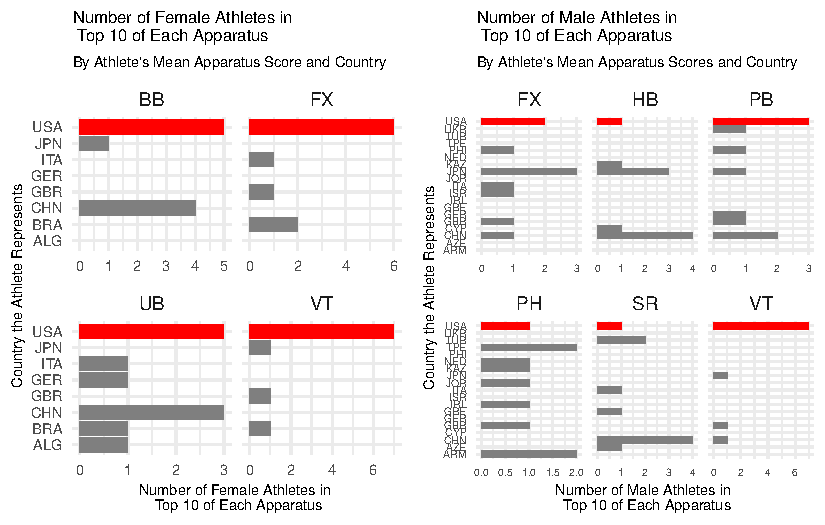
\includegraphics{Main_files/figure-pdf/top-10-athletes-1.pdf}

\hypertarget{methodology}{%
\section{Methodology}\label{methodology}}

Prior to conducting simulations, we cleaned our data set on the
2022-2023 gymnastics competition results. Our data set cleaning
semantics--wording, combining observations, etc. are in the appendix. We
then proceeded to minimize the number of observations in our data set
because we felt that it was unnecessary to simulate scores for athletes
that had little to no chance of ever medaling in the Olympics given
their previous records. To filter the observations, we first removed any
individual athletes entirely who had never made the finals in any event
in any competition in the data set. Afterward, we created quantiles of
20\% increments and 10\% increments for each round in a competition for
each apparatus, separated by gender because men and women compete
separately. We checked the number of unique athletes that competed at
each competition in each round (see Appendix), and found that for all
rounds in competitions other than the Oceania Championships, at least 36
unique athletes participated. For some rounds, hundreds of athletes
participated--so we decided to filter for: if more than 100 athletes
competed in a round in an apparatus, then we filtered for athletes'
scores in the top 10\%; if less than 100 athletes competed in a round in
an apparatus, then we filtered for athletes' scores in the top 20\%; for
the Oceania Championships, we filtered for the top 40\% (four athletes).
The reason we adopted a quantile-based filtering approach is because of
the variation in number of athletes who competed at different
competitions, so simply taking the top 20 athletes, for example, of each
competition may not account for that variation. Our last method of
filtering was to remove observations of athletes' scores for apparatuses
if an athlete had not competed more than twice in that apparatus in the
entire 2022-2023 data set. Our rationale was that there were 37 distinct
competitions in the data set, so if an athlete has not competed more
than twice in the past two years in an apparatus, they are likely not
that active in that apparatus. At this point, the issue arises that a
plurality of athletes has only ever done a single competition in any
given apparatus, resulting in a large number of athletes with 0
variances and skewing the distribution. Due to the unlikely nature of
athletes who do not compete regularly participating in the Olympics, we
have decided to truncate the apparatus level data set to exclude
athletes with less than three competition appearances for that given
apparatus. We are left with 2210 observations in our filtered data set
to conduct simulations, with 157 unique male athletes and 88 unique
female athletes.

\hypertarget{bayesian-monte-carlo-approach}{%
\subsection{Bayesian Monte Carlo
Approach}\label{bayesian-monte-carlo-approach}}

In this study, we present a Bayesian statistical Monte Carlo approach to
select the top male and female American gymnast candidates for
participation in the 2024 Olympics. Our method involves the creation of
prior distributions based on general historical performance data,
conditioning these distributions on individual competition results, and
simulating medal outcomes by predicting scores for each gymnast in each
apparatus event. This approach incorporates both prior beliefs and
observed data to make informed predictions about athletes' performances
in simulated events (Hoff, 2009). Utilizing Bayes' law for probability
density functions, where \(x\) is a vector of all the data from an
apparatus and gender combination, \(x_i\) represents the vector of
observed data for athlete \(i\), and \(\theta\) represents the
parameters of the distribution we will be using to model the
competition. We are under the assumption that all gymnastic scores are
independent and identically distributed for every athlete and that every
athlete's scores come from the same distribution type. Furthermore, for
modeling purposes, we assume a common prior \(p(x| \theta)\) for all
athletes such that \(p(x_i | \theta) = p(x| \theta)\) for all \(i\). Our
posterior distribution is:

\[
p(\theta |x_i) \propto p(x| \theta) p(\theta)
\]

To simulate a score for an athlete we sample
\(\theta^{(s)} \sim p(\theta | x_i)\) from the posterior and then sample
\(\tilde{x_i} \sim p(x| \theta^{(s)})\). This represents a new predicted
data point for athlete \(i\), a common practice for estimating values
from a posterior predictive distribution in Bayesian Monte Carlo
Simulations (Hoff, 2009). Thus, given we can simulate an athlete's
scores, we can then simulate a competition between all candidate
athletes and allocate gold, silver, and bronze medals to the top three
athletes.

\hypertarget{prior-distribution-creation-and-conditioning-on-individual-results}{%
\paragraph{Prior Distribution Creation and Conditioning on Individual
Results}\label{prior-distribution-creation-and-conditioning-on-individual-results}}

We began by creating prior distributions for each apparatus' total
score. See Exploratory Data Visualizations for the apparatus-gender
level distribution. Various distributions were considered, but the
normal distribution was chosen for ease of use and effective fit with
low standard errors and p-values \textless{} 0.01. We depended on
conjugacy to derive the parameters of the normal distribution. Since
both the mean and variance of the normal distribution are unknown, we
used a normal-inverse gamma prior.

To estimate prior parameters, we fit a normal distribution to the
distribution of athletes' means and an inverse-gamma distribution to
athletes' variances. We used the maximum likelihood method in the
\texttt{fitdist()} function (Muller, 2023). The maximum likelihood
estimates were then used as the prior parameters for the normal-inverse
gamma distribution. This process was done independently for all
apparatuses and genders. Following the establishment of the prior
distributions, we updated these distributions based on individuals'
competition results. We rely on existing literature for the formulas for
the posterior parameters (Hoff, 2009). We then employ a Monte Carlo
method to sample new data, simulating the posterior parameters for mean
and variance and then using these to simulate individual gymnastic
scores. See posterior predictive checks section in appendix for quality
of fit.

\hypertarget{simulation-of-gymnastics-events}{%
\paragraph{Simulation of Gymnastics
Events}\label{simulation-of-gymnastics-events}}

To simulate gymnastics events, we performed 500 iterations for each
apparatus event, resulting in about 11 million simulated scores. For
every iteration, we sampled a score for each athlete, \(\tilde{x_i}\),
from the posterior normal distribution. Furthermore, we truncated the
normal distribution at 0 and 20 to reflect the scoring system. We then
ranked the athletes by their simulated scores and awarded gold, silver,
and bronze medals to the top three athletes. Notably, we chose not to go
with a qualification structure and had a simple one-shot round for
victory. This decision was made due to computational constraints and was
accounted for when identifying Team USA athletes.

\hypertarget{assumptions}{%
\paragraph{Assumptions}\label{assumptions}}

We assume that gymnastic scores are normally distributed and
conditionally independent on the athlete. Additionally, we assume
independence between apparatus, allowing us to treat each apparatus
event as a separate and identically distributed random variable. We also
assumed that athletes prioritize all stages of every event identically.
Furthermore, we assume that historical performance data adequately
represents the gymnasts' true abilities and that changing age is not a
factor in gymnastic ability. While this assumption simplifies the
modeling process, it may not fully capture the complexities of
individual development and improvements over time.

\hypertarget{results}{%
\section{Results}\label{results}}

We ran simulations for each apparatus for each gender (women's 4
apparatuses and men's 6 apparatuses) 500 times, then outputted the top
athletes by medal count per apparatus.

\hypertarget{female-athletes-results}{%
\subsubsection{Female Athletes' Results}\label{female-athletes-results}}

For women's apparatuses, we outputted the tables of simulation outcomes
for floor exercise because of the high presence of medals for US
gymnasts. The table of simulation outcomes for other apparatuses are in
the appendix.

\begin{table}[H]

\caption{Women's Floor Exercise Simulation Results }
\centering
\fontsize{8}{10}\selectfont
\begin{tabular}[t]{l|r|r|r|r}
\hline
Athlete \& Country & Golds & Silvers & Bronzes & Total Medals\\
\hline
Simone Biles: USA & 186 & 85 & 57 & 328\\
\hline
Rebeca Andrade: BRA & 38 & 45 & 38 & 121\\
\hline
Kaliya Lincoln: USA & 30 & 37 & 29 & 96\\
\hline
Jessica Gadirova: GBR & 14 & 27 & 43 & 84\\
\hline
Flavia Saraiva: BRA & 27 & 25 & 18 & 70\\
\hline
Jade Carey: USA & 22 & 19 & 23 & 64\\
\hline
Martina Maggio: ITA & 11 & 18 & 29 & 58\\
\hline
Jordan Chiles: USA & 12 & 20 & 19 & 51\\
\hline
Joscelyn Roberson: USA & 10 & 17 & 20 & 47\\
\hline
Sabrina Maneca Voinea: ROU & 11 & 15 & 14 & 40\\
\hline
\end{tabular}
\end{table}

For the women's gymnastics team, we select Simone Biles, Zoe Miller,
Shilese Jones, Konnor McClain, and Jade Carey to represent the US at the
Paris Olympics. Our rationale for this combination and our framework for
optimizing gold medal count, total medal count, and apparatus
vs.~individual all-around vs.~team event wins are explored further in
the discussion.

Based on our 500 simulations, Simone Biles has the highest count of
total medals in balance beam (170 total medals), floor exercise (328
total medals), and vault (328 total medals), as well as highest gold
medal count in floor exercise and vault (186 and 151 gold medals
expected of 500 simulations, respectively). Therefore, Biles is expected
to be a strong US contender in the individual apparatus events,
individual all-around events, as well as a the team all-around since
only three members compete in each apparatus for that event. For uneven
bars, US athletes Zoe Miller and Shilese Jones come in third (35 gold
medals) and fifth place (32 gold medals) respectively. Additionally,
Konnor McClain comes second highest for gold medal count for balance
beam (65 gold medals) in simulation outcomes, after Yaqin Zhou of China,
and Jade Carey comes in third for highest count of total medals (199)
and gold medals (61 medals) for vault. Among the simulation results, we
generally see the US women gymnasts place very highly in individual
apparatuses by both total medal count and gold medal count.

\hypertarget{male-athletes-results}{%
\subsubsection{Male Athletes' Results}\label{male-athletes-results}}

For men's apparatuses, we outputted the table of simulation outcomes for
parallel bars because of the high presence of medals for US gymnasts
relative to the other apparatuses. The tables of simulation outcomes for
other apparatuses are in the appendix.

\begin{table}[H]

\caption{Men's Parallel Bars Simulation Results }
\centering
\fontsize{8}{10}\selectfont
\begin{tabular}[t]{l|r|r|r|r}
\hline
Athlete \& Country & Golds & Silvers & Bronzes & Total Medals\\
\hline
Jingyuan Zou: CHN & 133 & 75 & 49 & 257\\
\hline
Lukas Dauser: GER & 43 & 40 & 36 & 119\\
\hline
Boheng Zhang: CHN & 25 & 26 & 27 & 78\\
\hline
Curran Phillips: USA & 24 & 20 & 24 & 68\\
\hline
Colt Walker: USA & 20 & 28 & 19 & 67\\
\hline
Kaito Sugimoto: JPN & 23 & 25 & 17 & 65\\
\hline
Joe Fraser: GBR & 24 & 17 & 19 & 60\\
\hline
Carlos Yulo: PHI & 16 & 20 & 22 & 58\\
\hline
Cong Shi: CHN & 15 & 17 & 12 & 44\\
\hline
Blake Sun: USA & 15 & 10 & 19 & 44\\
\hline
\end{tabular}
\end{table}

For the men's gymnastics team, we select Asher Hong, Curran Phillips,
Donnell Whittenburg, Colt Walker, and Brody Malone to represent the US
at the Paris Olympics. Our rationale for choosing this combination and
optimizing for all-around gymnasts as opposed to event specialists are
explored further in the discussion.

We see from our simulation outcomes tables that the US men gymnasts do
not come in the top 3 simulated rankings by total medal count for any
apparatuses other than Asher Hong in vault, who comes in a simulated
second place. As a result, it may not be fruitful to pick individual US
male athletes by their apparatus-specific performance, given athletes
from other countries are likely to place ahead of them on individual
apparatuses. It is worth noting the overlap of US men gymnasts who place
in the top 10 of simulated total medals across the apparatuses. Curran
Phillips places in sixth in simulated total medals for vault (112
medals) and fourth in simulated total medals for parallel bars (68
medals). Donnell Whittenburg places seventh in simulated total medals
for still rings (56 medals), eighth for simulated total medals in floor
exercise (43 medals), and seventh for simulated total medals for vault
(111 medals). Colt Walker places ninth in simulated vault total medals
(85 medals), fifth in parallel bars simulated total medals (67 medals),
ninth in floor exercise simulated total medals (40 medals). Lastly,
Brody Malone places fourth in simulated high bar total medals (72
medals) and tenth in simulated floor exercise total medals (39 medals).
Because we see that these athletes are still able to place well in
multiple events, all the apparatuses except for pommel horse are covered
with at least one athlete who performs well in it, but who can also
place well in other apparatuses.

\hypertarget{discussion}{%
\section{Discussion}\label{discussion}}

\hypertarget{objective-1-choice-of-medal-success-metric-total-number-of-gold-medals}{%
\subsubsection{Objective 1: Choice of Medal Success Metric (Total Number
of Gold
Medals)}\label{objective-1-choice-of-medal-success-metric-total-number-of-gold-medals}}

From the dot plot visualizations of the women's simulation of the three
considered success metrics (gold medal count, total medal count, and
weighted medal count) for each apparatus by USA and non-USA teams, there
looks to be at least one USA athlete that places higher than of all
non-USA athletes in each medal metric for each apparatus except uneven
bars (Appendix: Image 5). The women's USA team makes up 51\% of the
total women's gold medals in the simulation which is a higher proportion
than the 47\% of the total medal count and 48\% of the weighted medals
(Appendix: Image 7). From the dot plot visualizations of the men's
simulation of the three considered success metrics, for each apparatus
by USA and non-USA teams, there are non-USA athletes for each apparatus
that exceed the USA in each medal success metric (Appendix: Image 6).
The men's USA team makes up 24\% of the total medal count in the
simulation which is a higher proportion than the 21\% of the total gold
medal count and 23\% of the weighted medals. (Appendix: Image 8) When
viewing the top 5 most successful female athletes (top 5 most decorated
by that medal metric) in each apparatus for each medal success metric,
the USA makes a good portion of these athletes. There tend to be 2-4 USA
athletes in the top 5 depending on the success metric and apparatus
(Appendix: Image 7). When viewing the top 5 most successful male
athletes in each apparatus for each medal success metric, there tend to
be 0-3 (mostly 0) US male athletes present (Appendix: Image 8).

Considering that US' female athletes tend to enjoy more successes,
regardless of metric, than male USA athletes, it is best to prioritize
the success metric that the female team performs the best in. Also
viewing the male top 5 most decorated athlete by each metric for each
apparatus, the men's USA team has a higher proportion of athletes in the
top 5 when using the total number of gold medals as a success metric
(Appendix: Image 8). Therefore, the success metric that we aim to
maximize to best ensure the USA team's success is the total number of
gold medals.

\hypertarget{objective-2-value-of-medals-for-each-event-type-team-aa-individual-aa-individual-apparatus}{%
\subsubsection{Objective 2: Value of Medals for Each Event Type (Team AA
\textgreater{} Individual AA \textgreater{} Individual
Apparatus)}\label{objective-2-value-of-medals-for-each-event-type-team-aa-individual-aa-individual-apparatus}}

From the table of the top 10 most decorated gold medal female athletes
by apparatus from the simulated data, the USA, China, Brazil, and Great
Britain make multiple appearances. The USA has athletes in the top 10
most decorated gold medalists for each apparatus as well as the top 5,
but other countries do not (Appendix: Image 9). In this case, valuing
the team's all-around medal more than the individual all-around and
individual apparatus will hopefully increase medal success in terms of
gold medal count. When viewing the top 10 most decorated gold medal
female athletes by apparatus, the USA's Simone Biles, appears in the
balance beam as first, in floor exercise as first, in uneven bars as
ninth, and in vault as first. Valuing the individual all-around events
higher also may help team USA increase in our metric of success.
Furthermore, since these events are harder to achieve than individual
apparatuses because of the multiple sections within the event that need
to also meet a standard, it will be harder for other countries to also
benefit from this increased value.

From the table of the top 10 most decorated gold medal male athletes by
apparatus, the USA, Japan, and China make multiple appearances. The only
country that has an athlete in each apparatus for the top 10, is the USA
(Appendix: Image 11). It could be beneficial for the men's team to value
the team's all-around success more than other events. The US men's team
also does not have a well-rounded athlete that places in the top 10 most
decorated gold male athletes for each apparatus so we can assume valuing
individual all-around successes over the other events would not help the
US men's team but it also would not hurt it since other countries also
do not have a highly decorated well-rounded competitor.

In the dot plots of the top 5 decorated gold medal female athletes'
countries by number of gold medals for each apparatus, US athletes make
multiple appearances (Appendix: Image 10). In the dot plots of the top 5
decorated gold medal male athlete's countries by number of gold medals
for each apparatus, US athletes are present in multiple apparatuses but
not many athletes are well decorated within each apparatus. But in vault
there are two US athletes in the top 5 (Appendix: Image 12). Valuing
individual apparatus events as regular events of weight 1 would best
suit both the male and female teams' success against their competitors.
Weighing the team all-around as 3 points is viable because not only do
both the men's and women's USA have the potential to win based on this
simulation, but there is less reliance on a single athlete.

\hypertarget{objective-3-all-around-vs-event-specialist-vs-mixture-women-even-specialist-men-mixture}{%
\subsubsection{Objective 3: All-Around vs Event Specialist vs Mixture
(Women: Even Specialist, Men:
Mixture)}\label{objective-3-all-around-vs-event-specialist-vs-mixture-women-even-specialist-men-mixture}}

In our metric of success, we chose the total count of gold medals and we
decided to weigh team all-around events as greater than individual
all-around events and individual all-around great than the individual
apparatuses. For the women's team, we believe it is best to select a
team of five female athletes who are event-specialist gymnasts. The US
women's team has a strong shot at winning the individual all-around and
many individual apparatus events with multiple-apparatus specialist as
well as win team all-around with highly decorated gold medalists who
specialize in their apparatus, so focusing on athletes that specialize
in apparatuses would be the best strategy (Appendix: Image 10). For the
men's team, we believe it is best to select a team of five male athletes
who are all-around gymnasts. The top male competitors for each apparatus
from Team USA are almost always severely overshadowed by top male
competitors from other countries by number of gold medal count. However,
in vault the US makes up 7 of the top 10 most decorated gold medalists
in the apparatus, so including as vault specialist could help the US
men's gymnastics team increase chances of success. (Appendix: Image 12)

\hypertarget{objective-4-identifying-5-athletes}{%
\subsubsection{Objective 4: Identifying 5
Athletes}\label{objective-4-identifying-5-athletes}}

Considering the conclusions of the previous objectives, we predict that
the following athletes would best optimize gold medal count success for
both the male and female US gymnastics team in the 2024 Paris Summer
Olympics:

\hypertarget{womens-usa-gymnastics-team-event-specialists-preference}{%
\paragraph{Women's USA Gymnastics Team: Event Specialists
Preference}\label{womens-usa-gymnastics-team-event-specialists-preference}}

Our Team USA women's selection includes: Simone Biles, Shilese Jones,
Zoe Miller, Konnor Mcclain, and Jade Carey.

In our results, we saw that Simone Biles was a strong individual
apparatus (particularly in floor exercise, vault, and balance beam),
individual all-around, and team all-around top-finisher contender--she
is both a specialist and a generalist. To supplement Biles's performance
and add strength to the US uneven bars performance, we choose Shilese
Jones and Zoe Miller for their strong uneven bars rankings as
specialists in the event. Furthermore, we choose Konnor McClain as a
specialist in balance beam, as she has more simulated gold medals than
does Simone Biles, but she may also compete on vault given fifth overall
simulated ranking in vault total medals and fourth overall simulated
ranking in vault gold medals. Lastly, Jade Carey we choose as another
vault specialist given her third overall simulated ranking in vault, but
she may also compete in floor exercise given her sixth overall simulated
medal ranking in floor exercise. This selection provides two of the
strongest USA specialists by medal count for almost each apparatus
besides floor exercise since Simone received a whopping count of 192
gold medals in comparison the second place Brazilian contender with 58
gold medals in the simulation (Appendix: Image 9).

\hypertarget{mens-usa-gymnastics-team-mixture-of-specialist-and-all-around-all-around-preference}{%
\paragraph{Men's USA Gymnastics Team: Mixture of Specialist and
All-Around, All-Around
Preference}\label{mens-usa-gymnastics-team-mixture-of-specialist-and-all-around-all-around-preference}}

Our Team USA men's selection includes: Asher Hong, Curran Phillips,
Donnell Whittenburg, Colt Walker, and Brody Malone.

In order to find the expected best all-around male athletes from the
simulation, we gave rankings of total count of gold medals for each
apparatus, took the average of those rankings for each athlete and
decided to pick the top five athletes with the highest average ranking
(Appendix: Image 13), but we will choose Curran Phillips as spot \#5
instead of Paul Juda given Curran Phillips places well in vault and
parallel bars, representing an all-arounder with additional specialties.
This method also matches our simulation results, which shows these five
athletes (except for Asher Hong as a vault specialist, yet Asher can
also rank high in all-around male athletes) as all-around gymnasts who
can place in the top 10 of simulated total medals in at least two
apparatuses, and cover all the apparatuses except for pommel horse.

\hypertarget{methodology-and-data-evaluation}{%
\subsubsection{Methodology and Data
Evaluation}\label{methodology-and-data-evaluation}}

The baseline choices in the methodology: taking a Bayesian approach and
relying on the Monte Carlo method, allow for generally informed
predictions (Yang, et. al 2022, Hoff 2008). However, there are areas
where the implementation could be improved. The normal distribution is a
simple choice for the posterior, but is not a perfect fit for the data.
The normal distribution is unbounded, while gymnastics scores are
bounded between 0 and 20. This discrepancy is addressed imperfectly
through truncation, while a beta distribution could potentially be a
better fit. Furthermore, when determining the prior parameters we use
the mean and standard deviation of athlete results in a given apparatus,
not accounting for the difference in sample count between athletes. We
use a single distribution to model final scores, when we should be
sampling from a distribution of difficulty scores, then conditioning on
difficulty to sample execution and penalty scores to get a final score.
This would allow us to incorporate the fact that difficulty and
execution scores are not independent. Additionally, the simulated
competitions include every gymnast in a single round, unlike the actual
Olympics. Ideally, we'd simulate the multiple individual and team rounds
in a gymnastics competition. The choice to avoid this modelling process,
alongside the choice to only run 500 simulations, were done due to
computational constraints. Finally, we assume that the athletes'
abilities are constant over time, which is not necessarily true. This
assumption is mildly addressed by using the most recent data, but it is
still a simplification.

We run our model on a subsetted group of observations from 2022-2023
gymnastics competition data; it is likely that this subset is not
representative of every athletes' true performances. We had to remove
data for athletes' scores when the athlete did not compete in more than
2 competitions for an apparatus, which may have excluded some injured or
upcoming athletes Finally, given there are a limited number of
international competitions per season, most athletes in the data set
were competing in less than ten competitions. The limited number of
score results per athlete may lead to hard to generalize results.

\hypertarget{implications-and-conclusions}{%
\subsubsection{Implications and
Conclusions}\label{implications-and-conclusions}}

A development of this study would be benefited if it addressed the
methodological limitations mentioned above. Additionally, including more
historical data and athletes' age in the model would create a much more
robust model. The current methodology also lacks a selection mechanism,
relying on us to manually select the top five athletes. Another change
that would have advanced the specificity in the vault apparatus scores
within our simulations would have been handling vault 1 and vault 2 as
separate entities. Within individual apparatus events, two different
vaults are required in the qualification and final event but in our
simulation we used the mean of both vault events instead. Another change
in our methodology would be to run more competition simulations to
reduce variance. Overall, this study provides valuable insights on an
optimal team selection strategy that would best aid the United States
artistic gymnastics male and female team achieve success in the 2024
Paris Summer Olympics Games.

\newpage

\hypertarget{appendix}{%
\section{Appendix}\label{appendix}}

\hypertarget{works-cited}{%
\subsubsection{Works Cited}\label{works-cited}}

\begin{itemize}
\item
  Camenker, Jacob. ``How Old Is Simone Biles? Why Elite Olympic Gymnasts
  Typically Retire at a Young Age.'' Sporting News, 18 Sept.~2021,
  www.sportingnews.com/us/athletics/news/simone-biles-retire-age-olympics/1laom4i4u4wh1thcgta4nun2x.
  Accessed 20 Nov.~2023.
\item
  Hoff, Peter D. A First Course in Bayesian Statistical Methods.
  Springer, 2009.
\item
  Meyers, Dvora. ``Time for the End of the Teen Gymnast.''
  FiveThirtyEight, 27 July 2021,
  fivethirtyeight.com/features/gymnasts-age-olympics/. Accessed 20
  Nov.~2023.
\item
  Muller, Marie Laure Delignette, and Christophe Dutang. ``Overview of
  the Fitdistrplus Package.'' R-Project, CRAN, 25 Apr.~2023,
  cran.r-project.org/web/packages/fitdistrplus/vignettes/fitdistrplus\_vignette.html.
\item
  ``Paris 2024 Olympic Games: How Do Athletes Qualify?'' Olympics, 8
  Aug.~2021,
  olympics.com/en/news/paris-2024-olympic-games-how-do-athletes-qualify.
  Accessed 20 Nov.~2023.
\item
  Santos-Fernandez, Edgar, et al.~``Bayesian Statistics Meets Sports: A
  Comprehensive Review.'' Journal of Quantitative Analysis in Sports,
  vol.~15, no. 4, Dec.~2019, pp.~289--312. www.degruyter.com,
  https://doi.org/10.1515/jqas-2018-0106.
\item
  ``Tokyo 2020 Artistic Gymnastics - Olympic Results by Discipline.''
  Olympics,
  olympics.com/en/olympic-games/tokyo-2020/results/artistic-gymnastics.
  Accessed 20 Nov.~2023.
\item
  ``UCSAS 2024 USOPC DATA CHALLENGE.'' UConn Sports Analytics Symposium
  (UCSAS), statds.org/events/ucsas2024/challenge.html. Accessed 20
  Nov.~2023.
\item
  Wu, Paul Pao-Yen, et. al.~(2021) Bayesian prediction of winning times
  for elite swimming events, Journal of Sports Sciences, 40:1, 24-31,
  DOI: 10.1080/02640414.2021.1976485
\end{itemize}

\hypertarget{data-discussion-tokyo-olympics}{%
\subsubsection{Data Discussion: Tokyo
Olympics}\label{data-discussion-tokyo-olympics}}

Additionally, in the context of Olympic gymnastics, athletes of age 16
and older are eligible to compete but gymnastics is a sport in which
most athletes retire in their early to mid-twenties. Specifically in the
summer 2020 Tokyo Olympics only three female athletes aged 27 or older
qualified to compete (Camenker, 2021). Furthermore, the average age for
female gymnasts in the 2020 Olympics was approximately 22 years of age,
meaning we assume that many of the competitors in the older data set
will not be competing in the 2024 Paris Summer Olympics (Meyers, 2021).

\hypertarget{data-cleaning-semantics-and-justification}{%
\subsubsection{Data Cleaning Semantics and
Justification}\label{data-cleaning-semantics-and-justification}}

There were several cases of missing or inconsistent athlete first and
last names, so we created unique athlete IDs using string methods by
using the first three letters of an athlete's first name, the first
three letters of an athlete's last name, and the country code. We also
manually inserted missing names and accounted for names with less than
three characters. Furthermore, the apparatus code for high bar was
inconsistent across the Commonwealth Games and all other competitions,
so we made sure to consolidate high bar into one apparatus code. Because
individual apparatus qualifying vaults needed athletes to compete in two
different vaults (VT1, VT2) as opposed to one vault in the finals or
team or all-around events, we decided to take the higher of the two
vault scores for an athlete for a competition, if there were two vaults
completed, and consolidated that score as one vault apparatus code. We
decided to keep the higher score given the vaults were different, and
athletes likely compete with the vault that gives them the higher score
during event finals.

\hypertarget{additional-simulation-results}{%
\subsubsection{Additional Simulation
Results}\label{additional-simulation-results}}

Given women compete on 4 apparatuses and men compete on 6 apparatuses,
we have tables of the simulation outcomes for all 10 apparatuses.

\begin{table}[H]

\caption{Women's Balance Beam Simulation Results }
\centering
\fontsize{8}{10}\selectfont
\begin{tabular}[t]{l|r|r|r|r}
\hline
Athlete \& Country & Golds & Silvers & Bronzes & Total Medals\\
\hline
Simone Biles: USA & 49 & 71 & 50 & 170\\
\hline
Yaqin Zhou: CHN & 68 & 49 & 42 & 159\\
\hline
Konnor McClain: USA & 65 & 47 & 29 & 141\\
\hline
Qingying Zhang: CHN & 54 & 32 & 41 & 127\\
\hline
Sunisa Lee: USA & 31 & 35 & 24 & 90\\
\hline
Huan Luo: CHN & 24 & 15 & 17 & 56\\
\hline
Yushan Ou: CHN & 12 & 21 & 17 & 50\\
\hline
Urara Ashikawa: JPN & 15 & 15 & 11 & 41\\
\hline
Rebeca Andrade: BRA & 11 & 14 & 13 & 38\\
\hline
Skye Blakely: USA & 10 & 12 & 16 & 38\\
\hline
\end{tabular}
\end{table}

\begin{table}[H]

\caption{Women's Vault Simulation Results }
\centering
\fontsize{8}{10}\selectfont
\begin{tabular}[t]{l|r|r|r|r}
\hline
Athlete \& Country & Golds & Silvers & Bronzes & Total Medals\\
\hline
Simone Biles: USA & 151 & 94 & 83 & 328\\
\hline
Rebeca Andrade: BRA & 103 & 79 & 63 & 245\\
\hline
Jade Carey: USA & 61 & 78 & 60 & 199\\
\hline
Jordan Chiles: USA & 28 & 34 & 43 & 105\\
\hline
Konnor McClain: USA & 40 & 32 & 31 & 103\\
\hline
Shilese Jones: USA & 22 & 38 & 39 & 99\\
\hline
Ondine Achampong: GBR & 14 & 31 & 46 & 91\\
\hline
Joscelyn Roberson: USA & 15 & 29 & 34 & 78\\
\hline
Shokyo Miyata: JPN & 26 & 21 & 30 & 77\\
\hline
Tiana Sumanasekera: USA & 18 & 31 & 26 & 75\\
\hline
\end{tabular}
\end{table}

\begin{table}[H]

\caption{Women's Uneven Bars Simulation Results }
\centering
\fontsize{9}{11}\selectfont
\begin{tabular}[t]{l|r|r|r|r}
\hline
Athlete \& Country & Golds & Silvers & Bronzes & Total Medals\\
\hline
Kayla Neymour: ALG & 82 & 55 & 42 & 179\\
\hline
Qiyan Qiu: CHN & 51 & 43 & 51 & 145\\
\hline
Shilese Jones: USA & 32 & 40 & 36 & 108\\
\hline
Alice D'Amato: ITA & 28 & 37 & 36 & 101\\
\hline
Xijing Tang: CHN & 33 & 29 & 30 & 92\\
\hline
Xiaoyuan Wei: CHN & 30 & 28 & 31 & 89\\
\hline
Zoe Miller: USA & 35 & 29 & 24 & 88\\
\hline
Rebeca Andrade: BRA & 22 & 19 & 21 & 62\\
\hline
Elisabeth Seitz: GER & 17 & 17 & 23 & 57\\
\hline
Simone Biles: USA & 15 & 16 & 21 & 52\\
\hline
\end{tabular}
\end{table}

\begin{table}[H]

\caption{Men's Vault Simulation Results }
\centering
\fontsize{8}{10}\selectfont
\begin{tabular}[t]{l|r|r|r|r}
\hline
Athlete \& Country & Golds & Silvers & Bronzes & Total Medals\\
\hline
Jake Jarman: GBR & 91 & 70 & 48 & 209\\
\hline
Asher Hong: USA & 67 & 58 & 58 & 183\\
\hline
Daiki Hashimoto: JPN & 55 & 55 & 46 & 156\\
\hline
Boheng Zhang: CHN & 54 & 44 & 37 & 135\\
\hline
Khoi Young: USA & 29 & 43 & 47 & 119\\
\hline
Curran Phillips: USA & 33 & 42 & 37 & 112\\
\hline
Donnell Whittenburg: USA & 35 & 38 & 38 & 111\\
\hline
Dallas Hale: USA & 34 & 29 & 47 & 110\\
\hline
Colt Walker: USA & 21 & 28 & 36 & 85\\
\hline
Taylor Burkhart: USA & 25 & 27 & 27 & 79\\
\hline
\end{tabular}
\end{table}

\begin{table}[H]

\caption{Men's Floor Exercise Simulation Results }
\centering
\fontsize{9}{11}\selectfont
\begin{tabular}[t]{l|r|r|r|r}
\hline
Athlete \& Country & Golds & Silvers & Bronzes & Total Medals\\
\hline
Carlos Yulo: PHI & 48 & 33 & 46 & 127\\
\hline
Ryosuke Doi: JPN & 26 & 26 & 31 & 83\\
\hline
Artem Dolgopyat: ISR & 21 & 22 & 26 & 69\\
\hline
Paul Juda: USA & 28 & 21 & 13 & 62\\
\hline
Daiki Hashimoto: JPN & 16 & 25 & 16 & 57\\
\hline
Boheng Zhang: CHN & 19 & 18 & 12 & 49\\
\hline
Nicola Bartolini: ITA & 13 & 18 & 12 & 43\\
\hline
Donnell Whittenburg: USA & 16 & 18 & 9 & 43\\
\hline
Colt Walker: USA & 16 & 13 & 12 & 41\\
\hline
Brody Malone: USA & 11 & 14 & 15 & 40\\
\hline
\end{tabular}
\end{table}

\begin{table}[H]

\caption{Men's High Bar Simulation Results }
\centering
\fontsize{9}{11}\selectfont
\begin{tabular}[t]{l|r|r|r|r}
\hline
Athlete \& Country & Golds & Silvers & Bronzes & Total Medals\\
\hline
Daiki Hashimoto: JPN & 44 & 45 & 35 & 124\\
\hline
Boheng Zhang: CHN & 50 & 26 & 33 & 109\\
\hline
Cong Shi: CHN & 35 & 38 & 27 & 100\\
\hline
Brody Malone: USA & 18 & 29 & 25 & 72\\
\hline
Weide Su: CHN & 23 & 20 & 16 & 59\\
\hline
Wei Sun: CHN & 26 & 20 & 13 & 59\\
\hline
Shohei Kawakami: JPN & 16 & 23 & 19 & 58\\
\hline
Ilias Georgiou: CYP & 18 & 15 & 20 & 53\\
\hline
Milad Karimi: KAZ & 25 & 11 & 15 & 51\\
\hline
Arthur Mariano: BRA & 11 & 19 & 16 & 46\\
\hline
\end{tabular}
\end{table}

\begin{table}[H]

\caption{Men's Pommel Horse Simulation Results }
\centering
\fontsize{9}{11}\selectfont
\begin{tabular}[t]{l|r|r|r|r}
\hline
Athlete \& Country & Golds & Silvers & Bronzes & Total Medals\\
\hline
Max Whitlock: GBR & 84 & 40 & 29 & 153\\
\hline
Chih Lee: TPE & 57 & 45 & 27 & 129\\
\hline
Nariman Kurbanov: KAZ & 31 & 52 & 35 & 118\\
\hline
Ahmad Abu Al Soud: JOR & 15 & 26 & 25 & 66\\
\hline
Rhys McClenaghan: IRL & 22 & 24 & 19 & 65\\
\hline
Stephen Nedoroscik: USA & 20 & 15 & 18 & 53\\
\hline
Loran De Munck: NED & 21 & 16 & 13 & 50\\
\hline
Gagik Khachikyan: ARM & 7 & 18 & 22 & 47\\
\hline
Yu-Jan Shiao: TPE & 11 & 16 & 18 & 45\\
\hline
Kakeru Tanigawa: JPN & 11 & 12 & 21 & 44\\
\hline
\end{tabular}
\end{table}

\begin{table}[H]

\caption{Men's Still Rings Simulation Results }
\centering
\fontsize{9}{11}\selectfont
\begin{tabular}[t]{l|r|r|r|r}
\hline
Athlete \& Country & Golds & Silvers & Bronzes & Total Medals\\
\hline
Yang Liu: CHN & 69 & 57 & 40 & 166\\
\hline
Xingyu Lan: CHN & 41 & 47 & 29 & 117\\
\hline
Eleftherious Petrounias: GRE & 38 & 34 & 36 & 108\\
\hline
Jingyuan Zou: CHN & 44 & 25 & 23 & 92\\
\hline
Hao You: CHN & 18 & 19 & 24 & 61\\
\hline
Ibrahim Colak: TUR & 18 & 22 & 18 & 58\\
\hline
Donnell Whittenburg: USA & 16 & 12 & 28 & 56\\
\hline
Adem Asil: TUR & 10 & 17 & 22 & 49\\
\hline
Salvatore Maresca: ITA & 12 & 24 & 13 & 49\\
\hline
Boheng Zhang: CHN & 17 & 19 & 9 & 45\\
\hline
\end{tabular}
\end{table}

\hypertarget{extra-visualizations}{%
\subsubsection{Extra Visualizations}\label{extra-visualizations}}

The following visualizations show the distribution of difficulty and
execution scores by apparatus for male and female gymnasts, which are
still approximately normal but do show more drastic deviations from
normality than do the overall scores for each gymnast at an apparatus in
a competition round. So, we thought it would be more fitting to fit
normal-inverse gamma priors on the means and variances of the overall
scores.

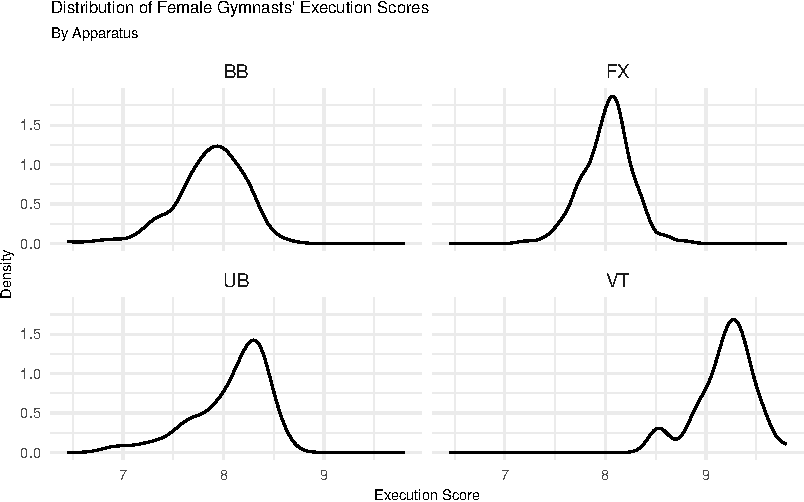
\includegraphics{Main_files/figure-pdf/execution-difficulty-distributions-1.pdf}

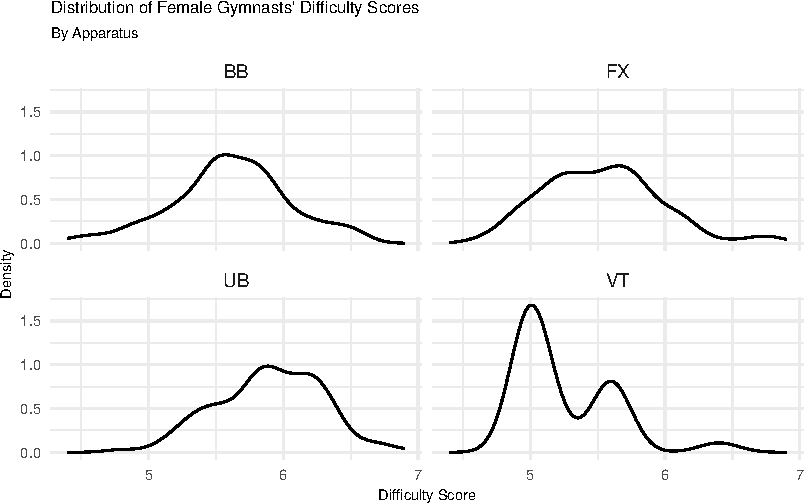
\includegraphics{Main_files/figure-pdf/execution-difficulty-distributions-2.pdf}

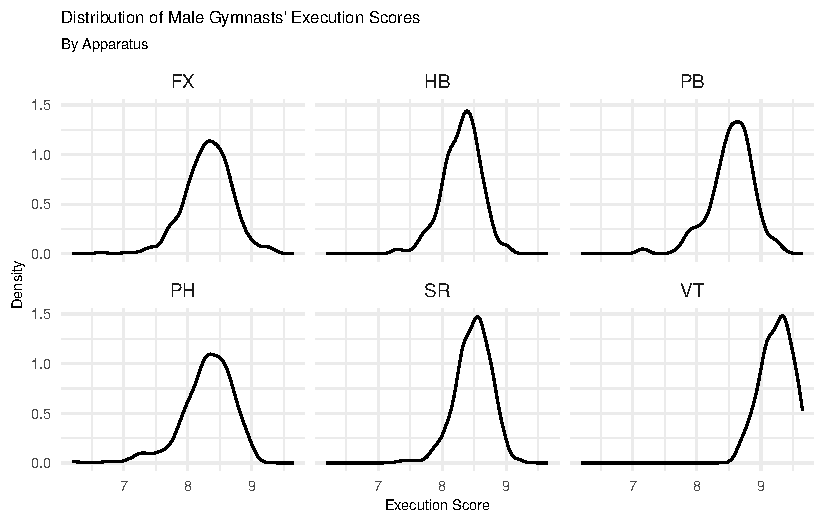
\includegraphics{Main_files/figure-pdf/execution-difficulty-distributions-3.pdf}

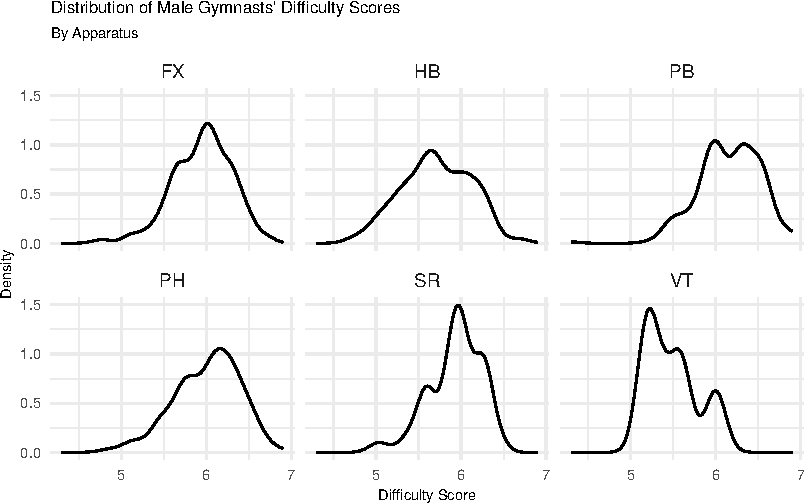
\includegraphics{Main_files/figure-pdf/execution-difficulty-distributions-4.pdf}

The below plots visualize how many unique athletes are competing at each
round in a competition, spearated by gender, so that we can understand
sample size for when we filter out data.

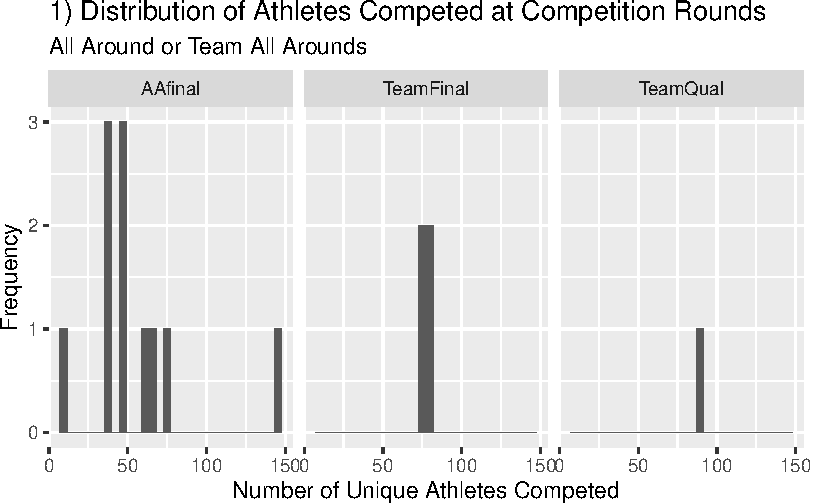
\includegraphics{Main_files/figure-pdf/unique-athletes-1.pdf}

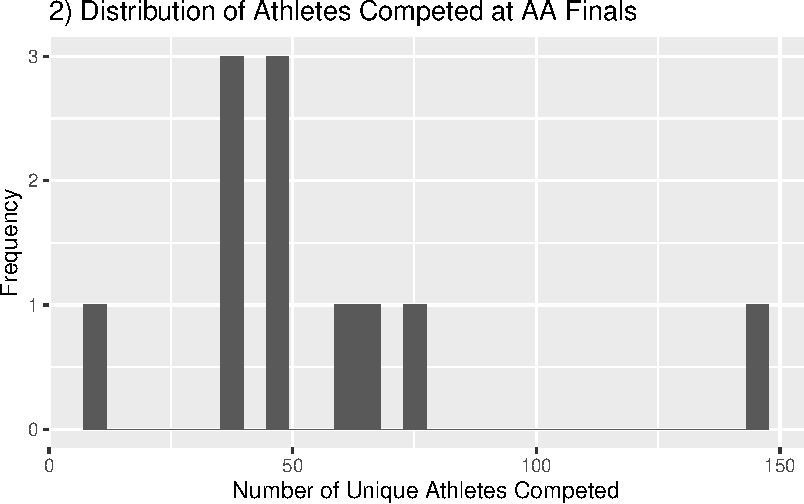
\includegraphics{Main_files/figure-pdf/unique-athletes-2.pdf}

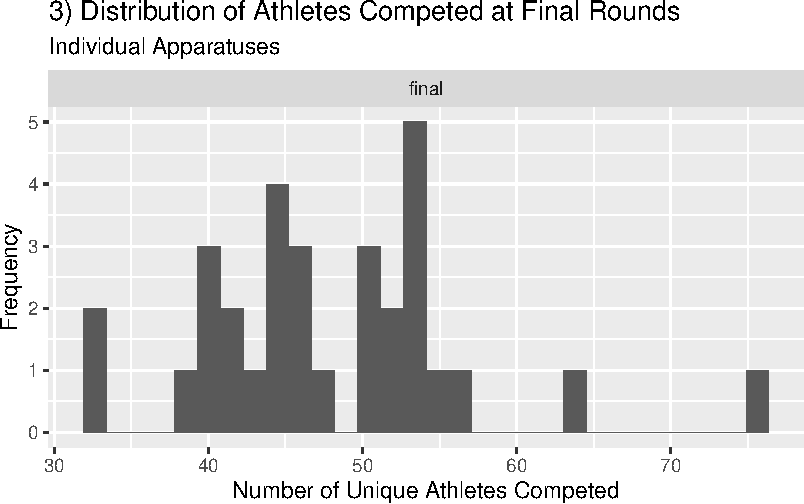
\includegraphics{Main_files/figure-pdf/unique-athletes-3.pdf}

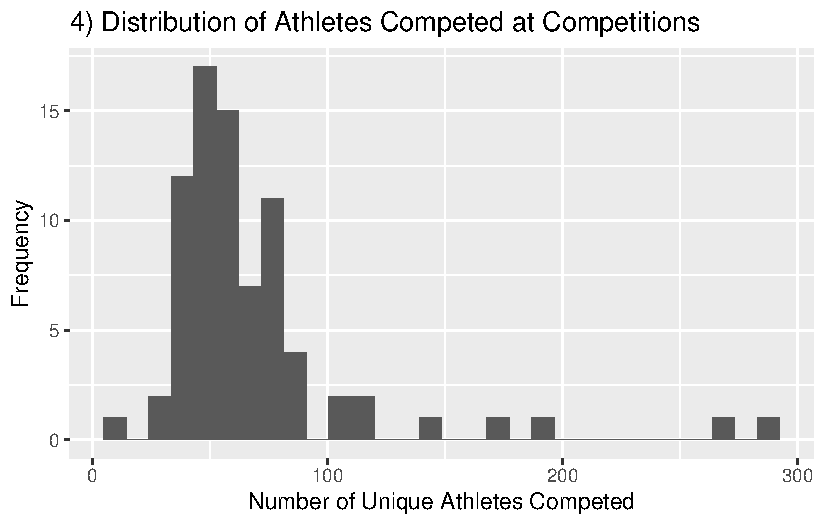
\includegraphics{Main_files/figure-pdf/unique-athletes-4.pdf}

\hypertarget{posterior-predictive-checks}{%
\subsubsection{Posterior Predictive
Checks}\label{posterior-predictive-checks}}

Additionally, we look to visualize the effectiveness of the choice of a
normal distribution by plotting MLE fitted normals over each apparatus.

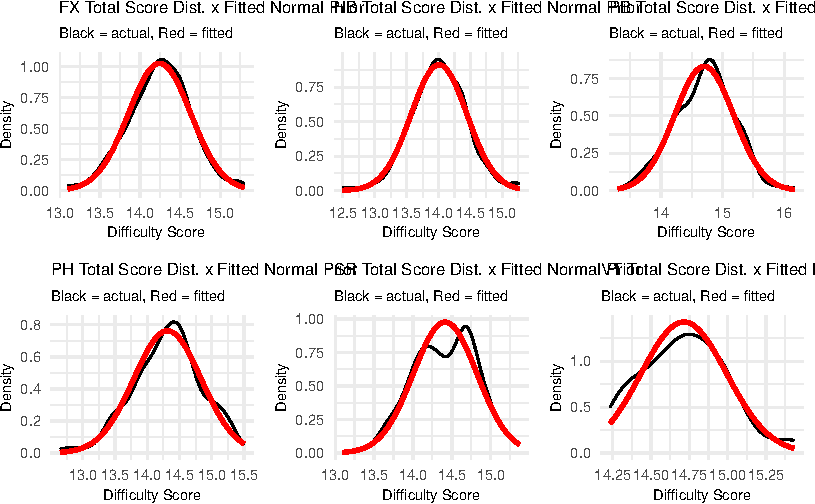
\includegraphics{Main_files/figure-pdf/unnamed-chunk-3-1.pdf}

And for the female events:

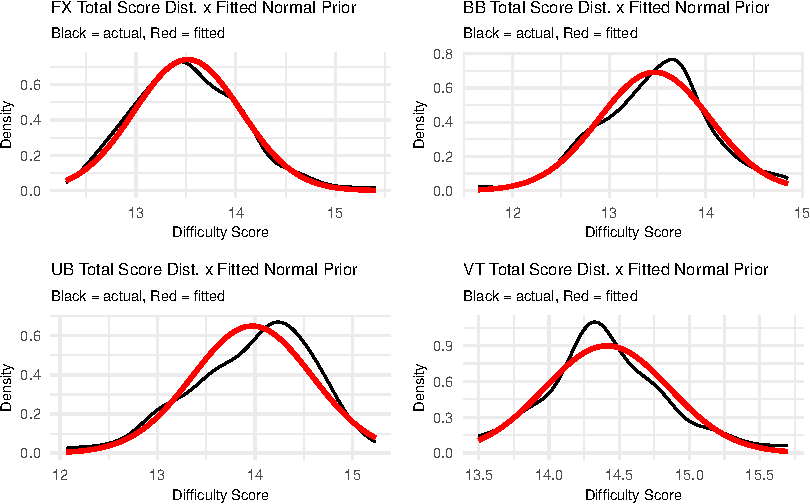
\includegraphics{Main_files/figure-pdf/unnamed-chunk-4-1.pdf}

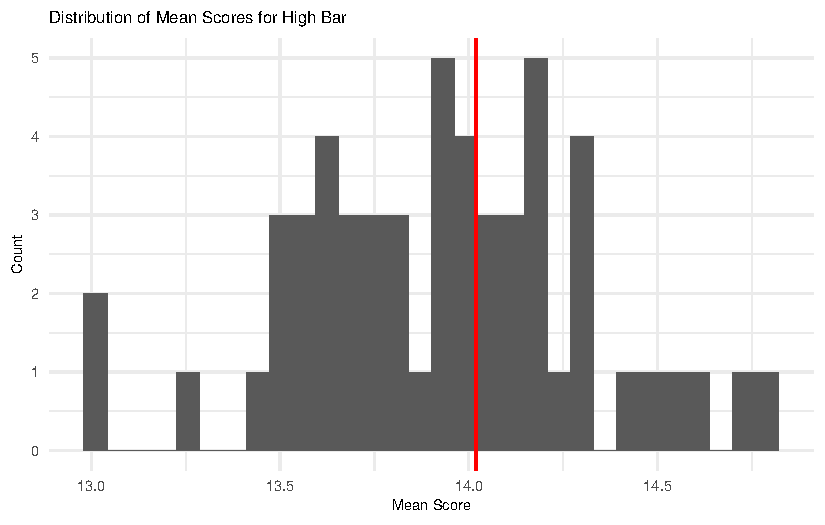
\includegraphics{Main_files/figure-pdf/scoremeans-var-1.pdf}

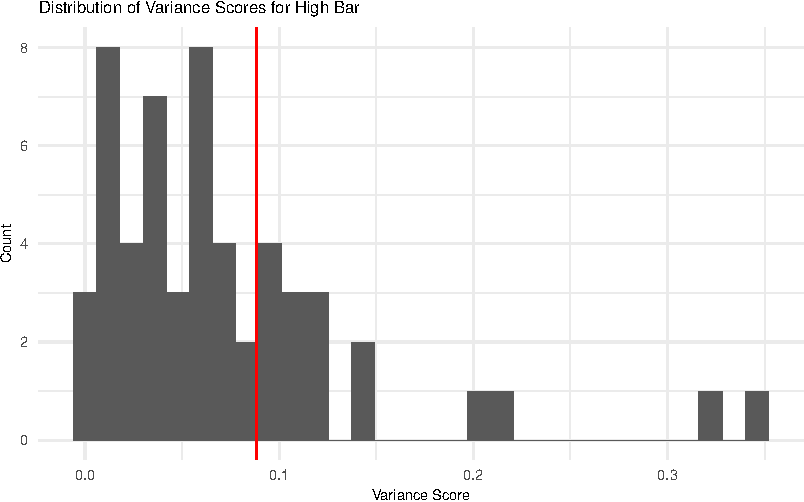
\includegraphics{Main_files/figure-pdf/scoremeans-var-2.pdf}

\hypertarget{comparing-simulation-results}{%
\subsubsection{Comparing Simulation
Results}\label{comparing-simulation-results}}

\textbf{Image 5)}

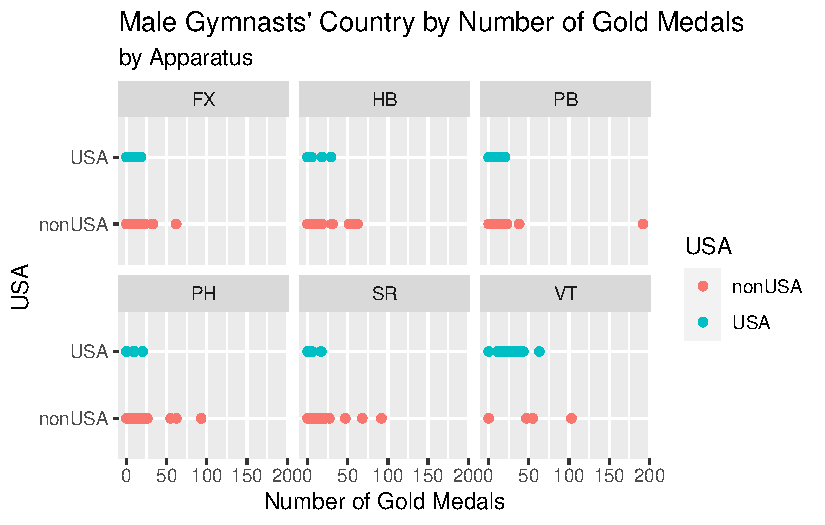
\includegraphics{Main_files/figure-pdf/unnamed-chunk-5-1.pdf}

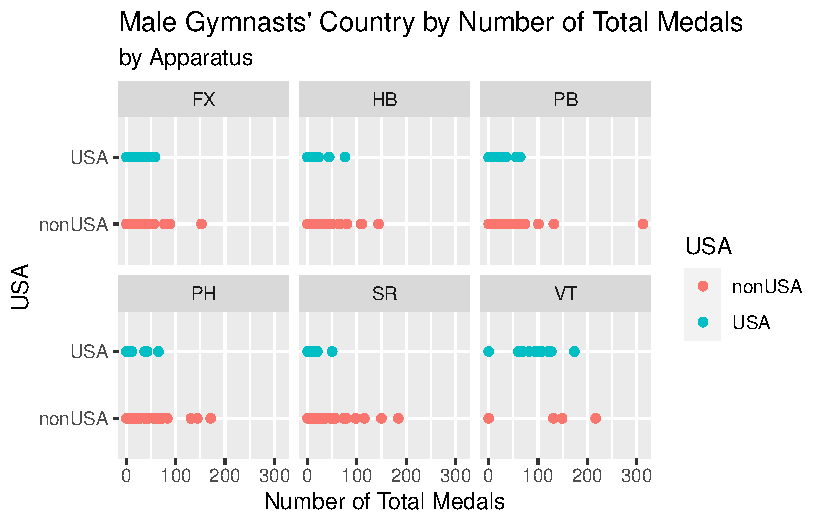
\includegraphics{Main_files/figure-pdf/unnamed-chunk-5-2.pdf}

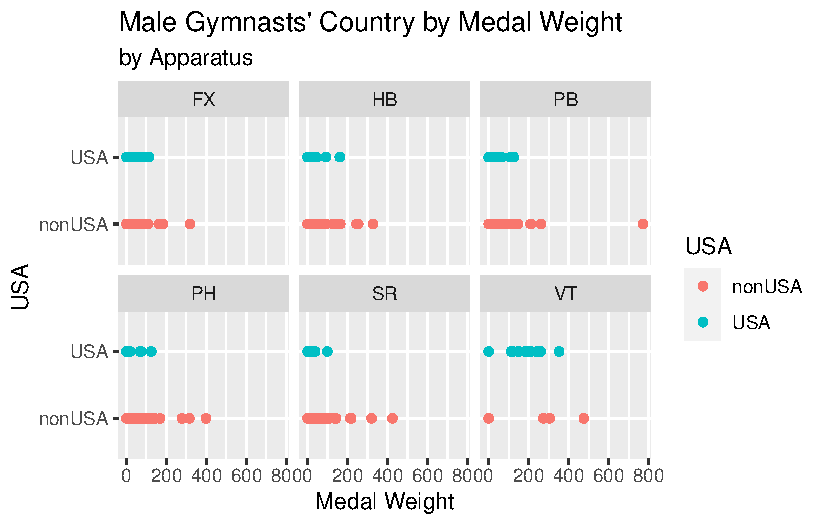
\includegraphics{Main_files/figure-pdf/unnamed-chunk-5-3.pdf}

\textbf{Image 6)}

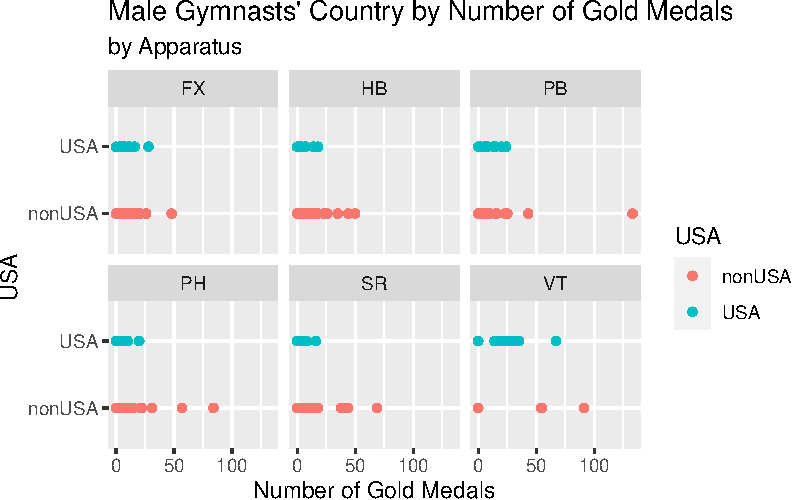
\includegraphics{Main_files/figure-pdf/unnamed-chunk-6-1.pdf}

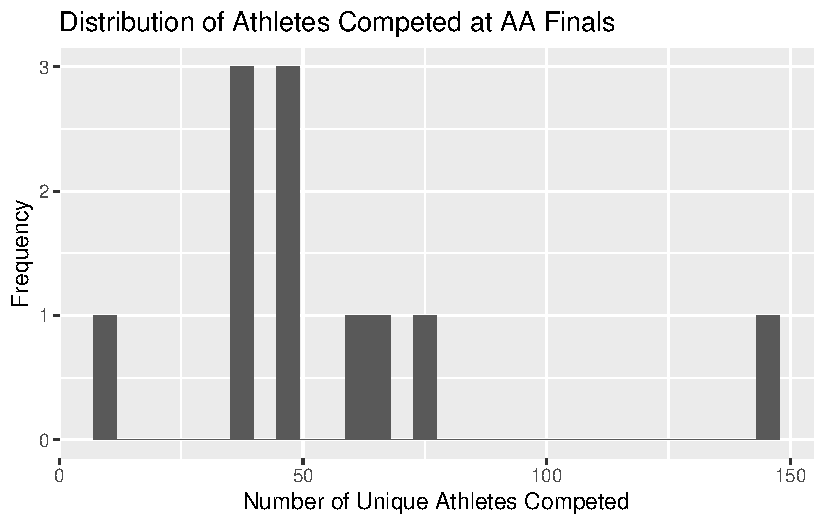
\includegraphics{Main_files/figure-pdf/unnamed-chunk-6-2.pdf}

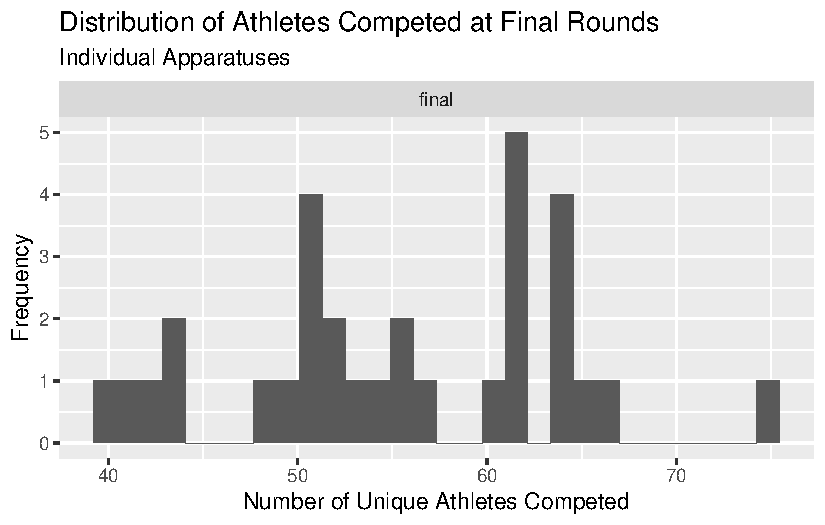
\includegraphics{Main_files/figure-pdf/unnamed-chunk-6-3.pdf}

\textbf{Image 7)}

Women:

\begin{itemize}
\item
  Top 5 athletes by apparatus for each of the 3 success metrics
\item
  Sum of each of the 3 metrics made by athletes from the US and non-US
  countries
\end{itemize}

\begin{table}[H]

\caption{Top Women's Athletes by Gold Medal Count}
\centering
\fontsize{8}{10}\selectfont
\begin{tabular}[t]{l|r|r|r|r|l|r|l|l}
\hline
Athlete \& Country & Golds & Silvers & Bronzes & Total Medals & Country & Medal Weight & Apparatus & Status\\
\hline
Yaqin Zhou: CHN & 68 & 49 & 42 & 159 & CHN & 344 & BB & nonUSA\\
\hline
Konnor McClain: USA & 65 & 47 & 29 & 141 & USA & 318 & BB & USA\\
\hline
Qingying Zhang: CHN & 54 & 32 & 41 & 127 & CHN & 267 & BB & nonUSA\\
\hline
Simone Biles: USA & 49 & 71 & 50 & 170 & USA & 339 & BB & USA\\
\hline
Sunisa Lee: USA & 31 & 35 & 24 & 90 & USA & 187 & BB & USA\\
\hline
Simone Biles: USA & 186 & 85 & 57 & 328 & USA & 785 & FX & USA\\
\hline
Rebeca Andrade: BRA & 38 & 45 & 38 & 121 & BRA & 242 & FX & nonUSA\\
\hline
Kaliya Lincoln: USA & 30 & 37 & 29 & 96 & USA & 193 & FX & USA\\
\hline
Flavia Saraiva: BRA & 27 & 25 & 18 & 70 & BRA & 149 & FX & nonUSA\\
\hline
Jade Carey: USA & 22 & 19 & 23 & 64 & USA & 127 & FX & USA\\
\hline
Kayla Neymour: ALG & 82 & 55 & 42 & 179 & ALG & 398 & UB & nonUSA\\
\hline
Qiyan Qiu: CHN & 51 & 43 & 51 & 145 & CHN & 290 & UB & nonUSA\\
\hline
Zoe Miller: USA & 35 & 29 & 24 & 88 & USA & 187 & UB & USA\\
\hline
Xijing Tang: CHN & 33 & 29 & 30 & 92 & CHN & 187 & UB & nonUSA\\
\hline
Shilese Jones: USA & 32 & 40 & 36 & 108 & USA & 212 & UB & USA\\
\hline
Simone Biles: USA & 151 & 94 & 83 & 328 & USA & 724 & VT & USA\\
\hline
Rebeca Andrade: BRA & 103 & 79 & 63 & 245 & BRA & 530 & VT & nonUSA\\
\hline
Jade Carey: USA & 61 & 78 & 60 & 199 & USA & 399 & VT & USA\\
\hline
Konnor McClain: USA & 40 & 32 & 31 & 103 & USA & 215 & VT & USA\\
\hline
Jordan Chiles: USA & 28 & 34 & 43 & 105 & USA & 195 & VT & USA\\
\hline
\end{tabular}
\end{table}

\begin{table}[H]

\caption{Top Women's Athletes by Total Medal Count}
\centering
\fontsize{8}{10}\selectfont
\begin{tabular}[t]{l|r|r|r|r|l|r|l|l}
\hline
Athlete \& Country & Golds & Silvers & Bronzes & Total Medals & Country & Medal Weight & Apparatus & Status\\
\hline
Simone Biles: USA & 49 & 71 & 50 & 170 & USA & 339 & BB & USA\\
\hline
Yaqin Zhou: CHN & 68 & 49 & 42 & 159 & CHN & 344 & BB & nonUSA\\
\hline
Konnor McClain: USA & 65 & 47 & 29 & 141 & USA & 318 & BB & USA\\
\hline
Qingying Zhang: CHN & 54 & 32 & 41 & 127 & CHN & 267 & BB & nonUSA\\
\hline
Sunisa Lee: USA & 31 & 35 & 24 & 90 & USA & 187 & BB & USA\\
\hline
Simone Biles: USA & 186 & 85 & 57 & 328 & USA & 785 & FX & USA\\
\hline
Rebeca Andrade: BRA & 38 & 45 & 38 & 121 & BRA & 242 & FX & nonUSA\\
\hline
Kaliya Lincoln: USA & 30 & 37 & 29 & 96 & USA & 193 & FX & USA\\
\hline
Jessica Gadirova: GBR & 14 & 27 & 43 & 84 & GBR & 139 & FX & nonUSA\\
\hline
Flavia Saraiva: BRA & 27 & 25 & 18 & 70 & BRA & 149 & FX & nonUSA\\
\hline
Kayla Neymour: ALG & 82 & 55 & 42 & 179 & ALG & 398 & UB & nonUSA\\
\hline
Qiyan Qiu: CHN & 51 & 43 & 51 & 145 & CHN & 290 & UB & nonUSA\\
\hline
Shilese Jones: USA & 32 & 40 & 36 & 108 & USA & 212 & UB & USA\\
\hline
Alice D'Amato: ITA & 28 & 37 & 36 & 101 & ITA & 194 & UB & nonUSA\\
\hline
Xijing Tang: CHN & 33 & 29 & 30 & 92 & CHN & 187 & UB & nonUSA\\
\hline
Simone Biles: USA & 151 & 94 & 83 & 328 & USA & 724 & VT & USA\\
\hline
Rebeca Andrade: BRA & 103 & 79 & 63 & 245 & BRA & 530 & VT & nonUSA\\
\hline
Jade Carey: USA & 61 & 78 & 60 & 199 & USA & 399 & VT & USA\\
\hline
Jordan Chiles: USA & 28 & 34 & 43 & 105 & USA & 195 & VT & USA\\
\hline
Konnor McClain: USA & 40 & 32 & 31 & 103 & USA & 215 & VT & USA\\
\hline
\end{tabular}
\end{table}

\begin{table}[H]

\caption{Top Women's Athletes by Weighted Medal Count}
\centering
\fontsize{8}{10}\selectfont
\begin{tabular}[t]{l|r|r|r|r|l|r|l|l}
\hline
Athlete \& Country & Golds & Silvers & Bronzes & Total Medals & Country & Medal Weight & Apparatus & Status\\
\hline
Yaqin Zhou: CHN & 68 & 49 & 42 & 159 & CHN & 344 & BB & nonUSA\\
\hline
Simone Biles: USA & 49 & 71 & 50 & 170 & USA & 339 & BB & USA\\
\hline
Konnor McClain: USA & 65 & 47 & 29 & 141 & USA & 318 & BB & USA\\
\hline
Qingying Zhang: CHN & 54 & 32 & 41 & 127 & CHN & 267 & BB & nonUSA\\
\hline
Sunisa Lee: USA & 31 & 35 & 24 & 90 & USA & 187 & BB & USA\\
\hline
Simone Biles: USA & 186 & 85 & 57 & 328 & USA & 785 & FX & USA\\
\hline
Rebeca Andrade: BRA & 38 & 45 & 38 & 121 & BRA & 242 & FX & nonUSA\\
\hline
Kaliya Lincoln: USA & 30 & 37 & 29 & 96 & USA & 193 & FX & USA\\
\hline
Flavia Saraiva: BRA & 27 & 25 & 18 & 70 & BRA & 149 & FX & nonUSA\\
\hline
Jessica Gadirova: GBR & 14 & 27 & 43 & 84 & GBR & 139 & FX & nonUSA\\
\hline
Kayla Neymour: ALG & 82 & 55 & 42 & 179 & ALG & 398 & UB & nonUSA\\
\hline
Qiyan Qiu: CHN & 51 & 43 & 51 & 145 & CHN & 290 & UB & nonUSA\\
\hline
Shilese Jones: USA & 32 & 40 & 36 & 108 & USA & 212 & UB & USA\\
\hline
Alice D'Amato: ITA & 28 & 37 & 36 & 101 & ITA & 194 & UB & nonUSA\\
\hline
Xijing Tang: CHN & 33 & 29 & 30 & 92 & CHN & 187 & UB & nonUSA\\
\hline
Zoe Miller: USA & 35 & 29 & 24 & 88 & USA & 187 & UB & USA\\
\hline
Simone Biles: USA & 151 & 94 & 83 & 328 & USA & 724 & VT & USA\\
\hline
Rebeca Andrade: BRA & 103 & 79 & 63 & 245 & BRA & 530 & VT & nonUSA\\
\hline
Jade Carey: USA & 61 & 78 & 60 & 199 & USA & 399 & VT & USA\\
\hline
Konnor McClain: USA & 40 & 32 & 31 & 103 & USA & 215 & VT & USA\\
\hline
Jordan Chiles: USA & 28 & 34 & 43 & 105 & USA & 195 & VT & USA\\
\hline
\end{tabular}
\end{table}

\begin{table}[H]

\caption{US Women's Medal Proportion Per Medal Metric}
\centering
\fontsize{8}{10}\selectfont
\begin{tabular}[t]{l|r|r|r}
\hline
Status & Sum Total Golds & Sum Total Medals & Sum Weighted Medals\\
\hline
nonUSA & 1040 & 3236 & 6380\\
\hline
USA & 960 & 2764 & 5620\\
\hline
\end{tabular}
\end{table}

For the women's simulation when looking at the top 5 athletes by:

\begin{itemize}
\item
  \emph{Gold Medal Count} for each apparatus there are 10 out of 20 from
  the US: balance beam (BB): 3, floor exercise (FX): 3, uneven bars
  (UB): 2, and vault (VT): 2

  \begin{itemize}
  \tightlist
  \item
    USA makes up 51\% of the total women's gold medals in the
    simulation.
  \end{itemize}
\item
  \emph{Total Medal Count} for each apparatus there are 12 out of 20
  from the US: balance beam (BB): 3, floor exercise (FX): 4, uneven bars
  (UB): 1, vault (VT): 4

  \begin{itemize}
  \tightlist
  \item
    USA makes up 47\% of the total women's medals in the simulation.
  \end{itemize}
\item
  \emph{Weighted Medal Count} for each apparatus there are 10 out of 20
  from the US: balance beam (BB): 3, floor exercise (FX): 2, uneven bars
  (UB): 1, vault (VT): 4

  \begin{itemize}
  \tightlist
  \item
    USA makes up 48\% of the weight of women's medals in the simulation.
  \end{itemize}
\end{itemize}

\textbf{Image 8)}

Men:

\begin{itemize}
\item
  Top 5 athletes by apparatus for each of the 3 success metrics
\item
  Sum of each of the 3 metrics made by athletes from the US and non-US
  countries
\end{itemize}

\begin{table}[H]

\caption{Top Men's Athletes by Gold Medal Count}
\centering
\fontsize{8}{10}\selectfont
\begin{tabular}[t]{l|r|r|r|r|l|r|l|l}
\hline
Athlete \& Country & Golds & Silvers & Bronzes & Total Medals & Country & Medal Weight & Apparatus & Status\\
\hline
Carlos Yulo: PHI & 48 & 33 & 46 & 127 & PHI & 256 & FX & nonUSA\\
\hline
Paul Juda: USA & 28 & 21 & 13 & 62 & USA & 139 & FX & USA\\
\hline
Ryosuke Doi: JPN & 26 & 26 & 31 & 83 & JPN & 161 & FX & nonUSA\\
\hline
Artem Dolgopyat: ISR & 21 & 22 & 26 & 69 & ISR & 133 & FX & nonUSA\\
\hline
Boheng Zhang: CHN & 19 & 18 & 12 & 49 & CHN & 105 & FX & nonUSA\\
\hline
Boheng Zhang: CHN & 50 & 26 & 33 & 109 & CHN & 235 & HB & nonUSA\\
\hline
Daiki Hashimoto: JPN & 44 & 45 & 35 & 124 & JPN & 257 & HB & nonUSA\\
\hline
Cong Shi: CHN & 35 & 38 & 27 & 100 & CHN & 208 & HB & nonUSA\\
\hline
Wei Sun: CHN & 26 & 20 & 13 & 59 & CHN & 131 & HB & nonUSA\\
\hline
Milad Karimi: KAZ & 25 & 11 & 15 & 51 & KAZ & 112 & HB & nonUSA\\
\hline
Jingyuan Zou: CHN & 133 & 75 & 49 & 257 & CHN & 598 & PB & nonUSA\\
\hline
Lukas Dauser: GER & 43 & 40 & 36 & 119 & GER & 245 & PB & nonUSA\\
\hline
Boheng Zhang: CHN & 25 & 26 & 27 & 78 & CHN & 154 & PB & nonUSA\\
\hline
Curran Phillips: USA & 24 & 20 & 24 & 68 & USA & 136 & PB & USA\\
\hline
Joe Fraser: GBR & 24 & 17 & 19 & 60 & GBR & 125 & PB & nonUSA\\
\hline
Max Whitlock: GBR & 84 & 40 & 29 & 153 & GBR & 361 & PH & nonUSA\\
\hline
Chih Lee: TPE & 57 & 45 & 27 & 129 & TPE & 288 & PH & nonUSA\\
\hline
Nariman Kurbanov: KAZ & 31 & 52 & 35 & 118 & KAZ & 232 & PH & nonUSA\\
\hline
Rhys McClenaghan: IRL & 22 & 24 & 19 & 65 & IRL & 133 & PH & nonUSA\\
\hline
Loran De Munck: NED & 21 & 16 & 13 & 50 & NED & 108 & PH & nonUSA\\
\hline
Yang Liu: CHN & 69 & 57 & 40 & 166 & CHN & 361 & SR & nonUSA\\
\hline
Jingyuan Zou: CHN & 44 & 25 & 23 & 92 & CHN & 205 & SR & nonUSA\\
\hline
Xingyu Lan: CHN & 41 & 47 & 29 & 117 & CHN & 246 & SR & nonUSA\\
\hline
Eleftherious Petrounias: GRE & 38 & 34 & 36 & 108 & GRE & 218 & SR & nonUSA\\
\hline
Hao You: CHN & 18 & 19 & 24 & 61 & CHN & 116 & SR & nonUSA\\
\hline
Ibrahim Colak: TUR & 18 & 22 & 18 & 58 & TUR & 116 & SR & nonUSA\\
\hline
Jake Jarman: GBR & 91 & 70 & 48 & 209 & GBR & 461 & VT & nonUSA\\
\hline
Asher Hong: USA & 67 & 58 & 58 & 183 & USA & 375 & VT & USA\\
\hline
Daiki Hashimoto: JPN & 55 & 55 & 46 & 156 & JPN & 321 & VT & nonUSA\\
\hline
Boheng Zhang: CHN & 54 & 44 & 37 & 135 & CHN & 287 & VT & nonUSA\\
\hline
Donnell Whittenburg: USA & 35 & 38 & 38 & 111 & USA & 219 & VT & USA\\
\hline
\end{tabular}
\end{table}

\begin{table}[H]

\caption{Top Men's Athletes by Total Medal Count}
\centering
\fontsize{8}{10}\selectfont
\begin{tabular}[t]{l|r|r|r|r|l|r|l|l}
\hline
Athlete \& Country & Golds & Silvers & Bronzes & Total Medals & Country & Medal Weight & Apparatus & Status\\
\hline
Carlos Yulo: PHI & 48 & 33 & 46 & 127 & PHI & 256 & FX & nonUSA\\
\hline
Ryosuke Doi: JPN & 26 & 26 & 31 & 83 & JPN & 161 & FX & nonUSA\\
\hline
Artem Dolgopyat: ISR & 21 & 22 & 26 & 69 & ISR & 133 & FX & nonUSA\\
\hline
Paul Juda: USA & 28 & 21 & 13 & 62 & USA & 139 & FX & USA\\
\hline
Daiki Hashimoto: JPN & 16 & 25 & 16 & 57 & JPN & 114 & FX & nonUSA\\
\hline
Daiki Hashimoto: JPN & 44 & 45 & 35 & 124 & JPN & 257 & HB & nonUSA\\
\hline
Boheng Zhang: CHN & 50 & 26 & 33 & 109 & CHN & 235 & HB & nonUSA\\
\hline
Cong Shi: CHN & 35 & 38 & 27 & 100 & CHN & 208 & HB & nonUSA\\
\hline
Brody Malone: USA & 18 & 29 & 25 & 72 & USA & 137 & HB & USA\\
\hline
Weide Su: CHN & 23 & 20 & 16 & 59 & CHN & 125 & HB & nonUSA\\
\hline
Wei Sun: CHN & 26 & 20 & 13 & 59 & CHN & 131 & HB & nonUSA\\
\hline
Jingyuan Zou: CHN & 133 & 75 & 49 & 257 & CHN & 598 & PB & nonUSA\\
\hline
Lukas Dauser: GER & 43 & 40 & 36 & 119 & GER & 245 & PB & nonUSA\\
\hline
Boheng Zhang: CHN & 25 & 26 & 27 & 78 & CHN & 154 & PB & nonUSA\\
\hline
Curran Phillips: USA & 24 & 20 & 24 & 68 & USA & 136 & PB & USA\\
\hline
Colt Walker: USA & 20 & 28 & 19 & 67 & USA & 135 & PB & USA\\
\hline
Max Whitlock: GBR & 84 & 40 & 29 & 153 & GBR & 361 & PH & nonUSA\\
\hline
Chih Lee: TPE & 57 & 45 & 27 & 129 & TPE & 288 & PH & nonUSA\\
\hline
Nariman Kurbanov: KAZ & 31 & 52 & 35 & 118 & KAZ & 232 & PH & nonUSA\\
\hline
Ahmad Abu Al Soud: JOR & 15 & 26 & 25 & 66 & JOR & 122 & PH & nonUSA\\
\hline
Rhys McClenaghan: IRL & 22 & 24 & 19 & 65 & IRL & 133 & PH & nonUSA\\
\hline
Yang Liu: CHN & 69 & 57 & 40 & 166 & CHN & 361 & SR & nonUSA\\
\hline
Xingyu Lan: CHN & 41 & 47 & 29 & 117 & CHN & 246 & SR & nonUSA\\
\hline
Eleftherious Petrounias: GRE & 38 & 34 & 36 & 108 & GRE & 218 & SR & nonUSA\\
\hline
Jingyuan Zou: CHN & 44 & 25 & 23 & 92 & CHN & 205 & SR & nonUSA\\
\hline
Hao You: CHN & 18 & 19 & 24 & 61 & CHN & 116 & SR & nonUSA\\
\hline
Jake Jarman: GBR & 91 & 70 & 48 & 209 & GBR & 461 & VT & nonUSA\\
\hline
Asher Hong: USA & 67 & 58 & 58 & 183 & USA & 375 & VT & USA\\
\hline
Daiki Hashimoto: JPN & 55 & 55 & 46 & 156 & JPN & 321 & VT & nonUSA\\
\hline
Boheng Zhang: CHN & 54 & 44 & 37 & 135 & CHN & 287 & VT & nonUSA\\
\hline
Khoi Young: USA & 29 & 43 & 47 & 119 & USA & 220 & VT & USA\\
\hline
\end{tabular}
\end{table}

\begin{table}[H]

\caption{Top Men's Athletes by Weighted Medal Count}
\centering
\fontsize{8}{10}\selectfont
\begin{tabular}[t]{l|r|r|r|r|l|r|l|l}
\hline
Athlete \& Country & Golds & Silvers & Bronzes & Total Medals & Country & Medal Weight & Apparatus & Status\\
\hline
Carlos Yulo: PHI & 48 & 33 & 46 & 127 & PHI & 256 & FX & nonUSA\\
\hline
Ryosuke Doi: JPN & 26 & 26 & 31 & 83 & JPN & 161 & FX & nonUSA\\
\hline
Paul Juda: USA & 28 & 21 & 13 & 62 & USA & 139 & FX & USA\\
\hline
Artem Dolgopyat: ISR & 21 & 22 & 26 & 69 & ISR & 133 & FX & nonUSA\\
\hline
Daiki Hashimoto: JPN & 16 & 25 & 16 & 57 & JPN & 114 & FX & nonUSA\\
\hline
Daiki Hashimoto: JPN & 44 & 45 & 35 & 124 & JPN & 257 & HB & nonUSA\\
\hline
Boheng Zhang: CHN & 50 & 26 & 33 & 109 & CHN & 235 & HB & nonUSA\\
\hline
Cong Shi: CHN & 35 & 38 & 27 & 100 & CHN & 208 & HB & nonUSA\\
\hline
Brody Malone: USA & 18 & 29 & 25 & 72 & USA & 137 & HB & USA\\
\hline
Wei Sun: CHN & 26 & 20 & 13 & 59 & CHN & 131 & HB & nonUSA\\
\hline
Jingyuan Zou: CHN & 133 & 75 & 49 & 257 & CHN & 598 & PB & nonUSA\\
\hline
Lukas Dauser: GER & 43 & 40 & 36 & 119 & GER & 245 & PB & nonUSA\\
\hline
Boheng Zhang: CHN & 25 & 26 & 27 & 78 & CHN & 154 & PB & nonUSA\\
\hline
Curran Phillips: USA & 24 & 20 & 24 & 68 & USA & 136 & PB & USA\\
\hline
Kaito Sugimoto: JPN & 23 & 25 & 17 & 65 & JPN & 136 & PB & nonUSA\\
\hline
Max Whitlock: GBR & 84 & 40 & 29 & 153 & GBR & 361 & PH & nonUSA\\
\hline
Chih Lee: TPE & 57 & 45 & 27 & 129 & TPE & 288 & PH & nonUSA\\
\hline
Nariman Kurbanov: KAZ & 31 & 52 & 35 & 118 & KAZ & 232 & PH & nonUSA\\
\hline
Rhys McClenaghan: IRL & 22 & 24 & 19 & 65 & IRL & 133 & PH & nonUSA\\
\hline
Ahmad Abu Al Soud: JOR & 15 & 26 & 25 & 66 & JOR & 122 & PH & nonUSA\\
\hline
Yang Liu: CHN & 69 & 57 & 40 & 166 & CHN & 361 & SR & nonUSA\\
\hline
Xingyu Lan: CHN & 41 & 47 & 29 & 117 & CHN & 246 & SR & nonUSA\\
\hline
Eleftherious Petrounias: GRE & 38 & 34 & 36 & 108 & GRE & 218 & SR & nonUSA\\
\hline
Jingyuan Zou: CHN & 44 & 25 & 23 & 92 & CHN & 205 & SR & nonUSA\\
\hline
Hao You: CHN & 18 & 19 & 24 & 61 & CHN & 116 & SR & nonUSA\\
\hline
Ibrahim Colak: TUR & 18 & 22 & 18 & 58 & TUR & 116 & SR & nonUSA\\
\hline
Jake Jarman: GBR & 91 & 70 & 48 & 209 & GBR & 461 & VT & nonUSA\\
\hline
Asher Hong: USA & 67 & 58 & 58 & 183 & USA & 375 & VT & USA\\
\hline
Daiki Hashimoto: JPN & 55 & 55 & 46 & 156 & JPN & 321 & VT & nonUSA\\
\hline
Boheng Zhang: CHN & 54 & 44 & 37 & 135 & CHN & 287 & VT & nonUSA\\
\hline
Khoi Young: USA & 29 & 43 & 47 & 119 & USA & 220 & VT & USA\\
\hline
Curran Phillips: USA & 33 & 42 & 37 & 112 & USA & 220 & VT & USA\\
\hline
\end{tabular}
\end{table}

\begin{table}[H]

\caption{US Men's Medal Proportion Per Medal Metric}
\centering
\fontsize{8}{10}\selectfont
\begin{tabular}[t]{l|r|r|r}
\hline
Status & Sum Total Golds & Sum Total Medals & Sum Weighted Medals\\
\hline
nonUSA & 2293 & 6667 & 13490\\
\hline
USA & 707 & 2333 & 4510\\
\hline
\end{tabular}
\end{table}

For the men's simulation when looking at the top 5 athletes by:

\begin{itemize}
\item
  \emph{Gold Medal Count} for each apparatus there are 5 out of 30 from
  the US: floor exercise (FX): 1, high bar (HB): 1, parallel bars (PB):
  1 pommel horse (PH): 0, still rings (SR): 0, vault (VT): 2

  \begin{itemize}
  \tightlist
  \item
    USA makes up 21\% of the total men's gold medals in the simulation.
  \end{itemize}
\item
  \emph{Total Medal Count} for each apparatus there are 4 out of 30 from
  the US: floor exercise (FX): 1, high bar (HB): 1, parallel bars (PB):
  0, pommel horse (PH): 0, still rings (SR): 0, vault (VT): 2

  \begin{itemize}
  \tightlist
  \item
    USA makes up 24\% of the total men's medals in the simulation.
  \end{itemize}
\item
  \emph{Weighted Medal Count} for each apparatus there are 4 out of 30
  from the US: floor exercise (FX): 1, high bar (HB): 1, parallel bars
  (PB): 0, pommel horse (PH): 0, still rings (SR): 0, vault (VT): 2

  \begin{itemize}
  \tightlist
  \item
    USA makes up 23\% of the weight of men's medals in the simulation.
  \end{itemize}
\end{itemize}

\textbf{Image 9)} Top ten most successful female gymnast using total
gold medal count by apparatus

\begin{table}[H]

\caption{Top 10 Female Athletes Per Apparatus by Gold Medals}
\centering
\fontsize{8}{10}\selectfont
\begin{tabular}[t]{l|r|l|l|l}
\hline
Athlete \& Country & Golds & Country & Apparatus & Status\\
\hline
Yaqin Zhou: CHN & 68 & CHN & BB & nonUSA\\
\hline
Konnor McClain: USA & 65 & USA & BB & USA\\
\hline
Qingying Zhang: CHN & 54 & CHN & BB & nonUSA\\
\hline
Simone Biles: USA & 49 & USA & BB & USA\\
\hline
Sunisa Lee: USA & 31 & USA & BB & USA\\
\hline
Huan Luo: CHN & 24 & CHN & BB & nonUSA\\
\hline
Urara Ashikawa: JPN & 15 & JPN & BB & nonUSA\\
\hline
Yushan Ou: CHN & 12 & CHN & BB & nonUSA\\
\hline
Shokyo Miyata: JPN & 12 & JPN & BB & nonUSA\\
\hline
Rebeca Andrade: BRA & 11 & BRA & BB & nonUSA\\
\hline
Emma Leonie Malewski: GER & 11 & GER & BB & nonUSA\\
\hline
Simone Biles: USA & 186 & USA & FX & USA\\
\hline
Rebeca Andrade: BRA & 38 & BRA & FX & nonUSA\\
\hline
Kaliya Lincoln: USA & 30 & USA & FX & USA\\
\hline
Flavia Saraiva: BRA & 27 & BRA & FX & nonUSA\\
\hline
Jade Carey: USA & 22 & USA & FX & USA\\
\hline
Konnor McClain: USA & 17 & USA & FX & USA\\
\hline
Jessica Gadirova: GBR & 14 & GBR & FX & nonUSA\\
\hline
Jordan Chiles: USA & 12 & USA & FX & USA\\
\hline
Martina Maggio: ITA & 11 & ITA & FX & nonUSA\\
\hline
Sabrina Maneca Voinea: ROU & 11 & ROU & FX & nonUSA\\
\hline
Yushan Ou: CHN & 11 & CHN & FX & nonUSA\\
\hline
Kayla Neymour: ALG & 82 & ALG & UB & nonUSA\\
\hline
Qiyan Qiu: CHN & 51 & CHN & UB & nonUSA\\
\hline
Zoe Miller: USA & 35 & USA & UB & USA\\
\hline
Xijing Tang: CHN & 33 & CHN & UB & nonUSA\\
\hline
Shilese Jones: USA & 32 & USA & UB & USA\\
\hline
Xiaoyuan Wei: CHN & 30 & CHN & UB & nonUSA\\
\hline
Alice D'Amato: ITA & 28 & ITA & UB & nonUSA\\
\hline
Rebeca Andrade: BRA & 22 & BRA & UB & nonUSA\\
\hline
Yunseo Lee: KOR & 19 & KOR & UB & nonUSA\\
\hline
Rebecca Downie: GBR & 19 & GBR & UB & nonUSA\\
\hline
Simone Biles: USA & 151 & USA & VT & USA\\
\hline
Rebeca Andrade: BRA & 103 & BRA & VT & nonUSA\\
\hline
Jade Carey: USA & 61 & USA & VT & USA\\
\hline
Konnor McClain: USA & 40 & USA & VT & USA\\
\hline
Jordan Chiles: USA & 28 & USA & VT & USA\\
\hline
Shokyo Miyata: JPN & 26 & JPN & VT & nonUSA\\
\hline
Shilese Jones: USA & 22 & USA & VT & USA\\
\hline
Tiana Sumanasekera: USA & 18 & USA & VT & USA\\
\hline
Skye Blakely: USA & 18 & USA & VT & USA\\
\hline
Joscelyn Roberson: USA & 15 & USA & VT & USA\\
\hline
\end{tabular}
\end{table}

\textbf{Image 10)}

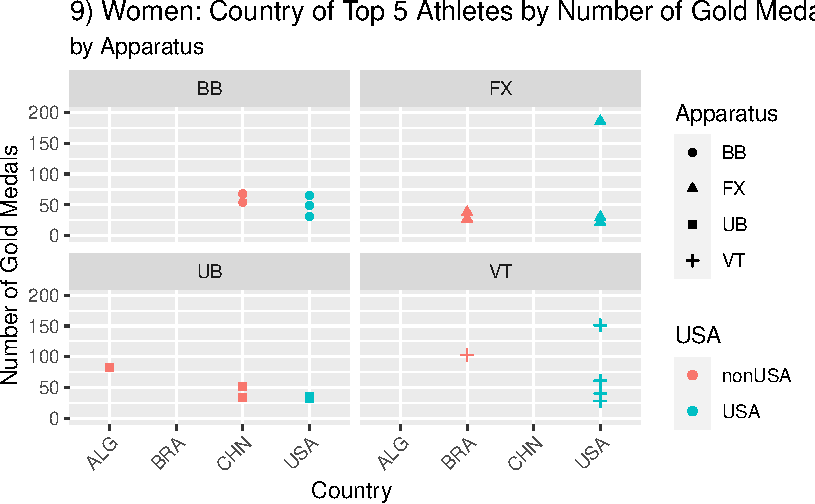
\includegraphics{Main_files/figure-pdf/unnamed-chunk-10-1.pdf}

\textbf{Image 11)} Top ten most successful male gymnast using total gold
medal count by apparatus

\begin{table}[H]

\caption{Top 10 Male Athletes Per Apparatus by Gold Medals}
\centering
\fontsize{8}{10}\selectfont
\begin{tabular}[t]{l|r|l|l|l}
\hline
Athlete \& Country & Golds & Country & Apparatus & Status\\
\hline
Carlos Yulo: PHI & 48 & PHI & FX & nonUSA\\
\hline
Paul Juda: USA & 28 & USA & FX & USA\\
\hline
Ryosuke Doi: JPN & 26 & JPN & FX & nonUSA\\
\hline
Artem Dolgopyat: ISR & 21 & ISR & FX & nonUSA\\
\hline
Boheng Zhang: CHN & 19 & CHN & FX & nonUSA\\
\hline
Daiki Hashimoto: JPN & 16 & JPN & FX & nonUSA\\
\hline
Donnell Whittenburg: USA & 16 & USA & FX & USA\\
\hline
Colt Walker: USA & 16 & USA & FX & USA\\
\hline
Hansol Kim: KOR & 15 & KOR & FX & nonUSA\\
\hline
William Emard: CAN & 15 & CAN & FX & nonUSA\\
\hline
Boheng Zhang: CHN & 50 & CHN & HB & nonUSA\\
\hline
Daiki Hashimoto: JPN & 44 & JPN & HB & nonUSA\\
\hline
Cong Shi: CHN & 35 & CHN & HB & nonUSA\\
\hline
Wei Sun: CHN & 26 & CHN & HB & nonUSA\\
\hline
Milad Karimi: KAZ & 25 & KAZ & HB & nonUSA\\
\hline
Weide Su: CHN & 23 & CHN & HB & nonUSA\\
\hline
Brody Malone: USA & 18 & USA & HB & USA\\
\hline
Ilias Georgiou: CYP & 18 & CYP & HB & nonUSA\\
\hline
Shohei Kawakami: JPN & 16 & JPN & HB & nonUSA\\
\hline
Frederick Richard USA & 14 & USA & HB & USA\\
\hline
Chaopan Lin: CHN & 14 & CHN & HB & nonUSA\\
\hline
Jingyuan Zou: CHN & 133 & CHN & PB & nonUSA\\
\hline
Lukas Dauser: GER & 43 & GER & PB & nonUSA\\
\hline
Boheng Zhang: CHN & 25 & CHN & PB & nonUSA\\
\hline
Curran Phillips: USA & 24 & USA & PB & USA\\
\hline
Joe Fraser: GBR & 24 & GBR & PB & nonUSA\\
\hline
Kaito Sugimoto: JPN & 23 & JPN & PB & nonUSA\\
\hline
Colt Walker: USA & 20 & USA & PB & USA\\
\hline
Carlos Yulo: PHI & 16 & PHI & PB & nonUSA\\
\hline
Cong Shi: CHN & 15 & CHN & PB & nonUSA\\
\hline
Blake Sun: USA & 15 & USA & PB & USA\\
\hline
Max Whitlock: GBR & 84 & GBR & PH & nonUSA\\
\hline
Chih Lee: TPE & 57 & TPE & PH & nonUSA\\
\hline
Nariman Kurbanov: KAZ & 31 & KAZ & PH & nonUSA\\
\hline
Rhys McClenaghan: IRL & 22 & IRL & PH & nonUSA\\
\hline
Loran De Munck: NED & 21 & NED & PH & nonUSA\\
\hline
Stephen Nedoroscik: USA & 20 & USA & PH & USA\\
\hline
Ahmad Abu Al Soud: JOR & 15 & JOR & PH & nonUSA\\
\hline
Jamie Lewis: GBR & 13 & GBR & PH & nonUSA\\
\hline
Daiki Hashimoto: JPN & 13 & JPN & PH & nonUSA\\
\hline
Dehang Yin: CHN & 13 & CHN & PH & nonUSA\\
\hline
Yang Liu: CHN & 69 & CHN & SR & nonUSA\\
\hline
Jingyuan Zou: CHN & 44 & CHN & SR & nonUSA\\
\hline
Xingyu Lan: CHN & 41 & CHN & SR & nonUSA\\
\hline
Eleftherious Petrounias: GRE & 38 & GRE & SR & nonUSA\\
\hline
Hao You: CHN & 18 & CHN & SR & nonUSA\\
\hline
Ibrahim Colak: TUR & 18 & TUR & SR & nonUSA\\
\hline
Boheng Zhang: CHN & 17 & CHN & SR & nonUSA\\
\hline
Nikita Simonov: AZE & 17 & AZE & SR & nonUSA\\
\hline
Donnell Whittenburg: USA & 16 & USA & SR & USA\\
\hline
Mahdi Ahmad Kohani: IRI & 15 & IRI & SR & nonUSA\\
\hline
Jake Jarman: GBR & 91 & GBR & VT & nonUSA\\
\hline
Asher Hong: USA & 67 & USA & VT & USA\\
\hline
Daiki Hashimoto: JPN & 55 & JPN & VT & nonUSA\\
\hline
Boheng Zhang: CHN & 54 & CHN & VT & nonUSA\\
\hline
Donnell Whittenburg: USA & 35 & USA & VT & USA\\
\hline
Dallas Hale: USA & 34 & USA & VT & USA\\
\hline
Curran Phillips: USA & 33 & USA & VT & USA\\
\hline
Khoi Young: USA & 29 & USA & VT & USA\\
\hline
Taylor Burkhart: USA & 25 & USA & VT & USA\\
\hline
Kameron Nelson: USA & 23 & USA & VT & USA\\
\hline
\end{tabular}
\end{table}

\textbf{Image 12)}

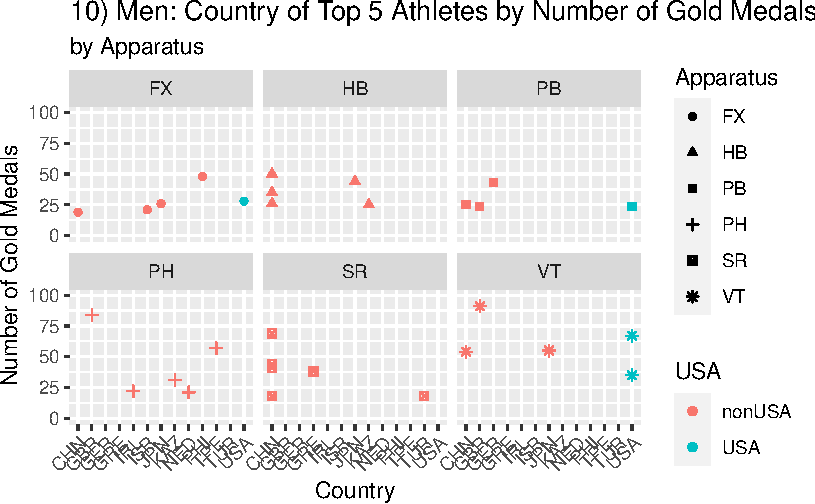
\includegraphics{Main_files/figure-pdf/top5-decorated-1.pdf}

\textbf{\emph{Note:}} The excessive number of countries display that
there is not much overlap in the top 5 most gold medal decorated
athletes on the men's team and therefore the lack of well-rounded
gymnasts.

\textbf{Image 13)}

Average of total gold medal count ranking by apparatus of all US male
gymnasts in ascending order -- lower average rank meaning better
results, that is, placing higher in rank. We output this average rank in
order to find best all around gymnast for men's team.

\begin{table}[H]

\caption{Top 10 Average Ranks of USA Male Athletes By Number of Gold Medals}
\centering
\fontsize{8}{10}\selectfont
\begin{tabular}[t]{l|r}
\hline
Athlete \& Country & Average Rank\\
\hline
Donnell Whittenburg: USA & 13.66667\\
\hline
Asher Hong: USA & 14.00000\\
\hline
Brody Malone: USA & 14.00000\\
\hline
Colt Walker: USA & 14.33333\\
\hline
Paul Juda: USA & 15.50000\\
\hline
Curran Phillips: USA & 15.66667\\
\hline
Frederick Richard: USA & 16.00000\\
\hline
Khoi Young: USA & 16.16667\\
\hline
Shane Wiskus: USA & 16.83333\\
\hline
Yul Moldauer: USA & 17.00000\\
\hline
\end{tabular}
\end{table}



\end{document}
